\section{Faithful Generation Through Data-Augmentation: Noise-Injection Sampling and Self-Training}
\label{sec:nlgfg}

We now formally define faithfulness as it relates to the
\meaningrepresentation~to text generation problem.  Let $\GEN : \mrspace
\rightarrow \outSpace$ be an arbitrary mapping from \meaningrepresentations~to
utterances. We say that a mapping $\GEN$ is \faithful~if \[\denotes{\GEN(\mr)}
= \mr \quad \forall \mr: \mr \in \mrspace.\] In words, $\GEN$ is faithful if
the propositional content of $\mr$ (i.e., the semantics of the
\attributevalue~pairs in $\mr$) is correctly expressed by the generated
utterance $\predutttoks = \GEN(\mr)$ for any well-formed
\meaningrepresentation~$\mr$. 

If $\GEN$ is implemented with templates as in \cite{puzikov2018}, it is
possible to design a faithful mapping. However, it is possible that
faithfulness and naturalness are in tension, as the method of
\cite{puzikov2018} did not perform as highly on human judgements of
naturalness.

It is well known that implementing $\GEN$ with a neural model $\gen$ and an
inference procedure such as beam search are not sufficient to obtain a faithful
model.  Beam search, which only expands candidates whose next word
continuations are highly probable, tends to produce low-perplexity utterances
\citep{serban2016}. Low-perplexity utterances may satisfy perceived notions of
quality \citep{meister2020}, but this is not a sufficient condition for
semantic correctness.  As mentioned in \autoref{sec:nlginference},  a common
approach to make $\gen$ more faithful is to perform overgeneration with
reranking \citep{dusek2016,juraska2018,dusek2019,dusek2020}.  The $\nbest$-best
list of utterances $\mathcal{H}_{complete} = \left\{\utttoks^{(1)},\ldots,
\utttoks^{(\nbest)}\right\}$ is produced using beam search with
$\gen\left(\cdot|\ls(\mr)\right).$ Then a discriminative
\meaningrepresentation~parser, $\dmodel(\cdot|\cdot) : \mrspace \times
\outSpace \rightarrow (0,1)$, is used to rerank $\mathcal{H}_{complete}$ such
that the final output utterance is \[ \predutttoks = \argmax_{\utttoks \in
\mathcal{H}_{complete}} \dmodel\left(\mr\vert\utttoks\right). \] In this
setting the inference procedure selects the utterance that most likely denotes
the input $\mr$ under $\dmodel$. While this reduces the risk of generating an
incorrect utterance with respect to $\mr$, it can still fail when either
$\dmodel$ is not accurate or when $\mathcal{H}_{complete}$ does not contain a
completely correct utterance.

The critical issue here is that the final beam search hypothesis set may not
contain any completely semantically correct utterances.  This in part happens
because neural models on natural language data\footnote{Here we are referring
to both \sequencetosequence~models but also sequence classification
\citep{kim2014convolutional,mccoy2019} and sequence-pair classification
\citep{he2019}. }  do not na{\"i}vely exhibit the quality of systematicity
\citep{fodor1988,phillips1998,marcus2003,lake18,mccoy2019,gardner2020}. A model
displays systematicity if the capability of the model to  perform a task
implies that it can perform other structurally related tasks successfully.  On
natural language data, a model with systematicity should be able to exploit the
algebraic and compositional nature of natural language to make correct
inferences. \citet{lake18} give the example of a human speaker that understands
the concept of ``twice'' or ``again,'' who, upon learning a novel verb, ``to
dax,'' immediately understands the meaning of ``daxed twice'' or ``to dax
again'' even though they have never seen examples of these compositions before.
Empirically, they demonstrate that a \recurrentneuralnetwork~based
text-to-\meaningrepresentation~model  does not possess this ability and
frequently fails to generalize to novel compositions even where the individual
constituents of the compositions are well represented in the training data.
\cite{bastings2018} show that this also holds going the other direction, from
\meaningrepresentation~to text, the more relevant direction for our present
discussion.

In our case, this lack of systematicity manifests itself as a failure to
realize individual \attributevalues~that are well represented in the training
data when those \attributevalues~occur in novel combinations in a
\meaningrepresentation~at test time. We use as a case-study, the
\attributevalue~\textit{near=Burger King}. which in our restaurant domain
dataset, the E2E Challenge dataset \citep{dusek2018}, denotes that a restaurant
$x$ is near Burger King. 

The \attributevalue~\textit{near=Burger King} appears frequently in the
training data in longer \meaningrepresentation/utterance pairs. In fact
\textit{near=Burger King} is positively associated with
\meaningrepresentations~where seven or eight \attributes~are specified (there
are eight total unique attributes on this dataset). See \autoref{fig:bkpmi}
where we plot the point-wise mutual information (PMI) \citep{church1990} of the
occurrence of the \textit{near=Burger King} and the occurrence of a
\meaningrepresentation~of a particular size on the training set, where the size
of a \meaningrepresentation~$\setsize{\mr}$ is the number of
\attributevalue~pairs in $\mr$.  The PMI is computed as 
\[\pmi(\AV{near}{Burger King},  \setsize{\mr} = k) = \log \frac{p(\AV{near}{Burger King}, \setsize{\mr} = k)}{p( \AV{near}{Burger King}  ) p(\setsize{\mr} = k)}     \quad \forall k : k \in \{3,\ldots,8\},\]
with \begin{align*}
    p(\AV{near}{Burger King}) &= \frac{\sum_{(\mr,\utttoks) \in \corpus}\mathds{1}\left\{ \AV{near}{Burger King} \in \mr \right\}}{\setsize{\corpus}} \\
    p(\setsize{\mr}=k) &= \frac{\sum_{(\mr,\utttoks) \in \corpus}\mathds{1}\left\{ \setsize{\mr} = k \right\}}{\setsize{\corpus}} \\
    p(\AV{near}{Burger King},\setsize{\mr}=k) &= \frac{\sum_{(\mr,\utttoks) \in \corpus}\mathds{1}\left\{\AV{near}{Burger King} \in \mr \wedge \setsize{\mr} = k \right\}}{\setsize{\corpus}}.
\end{align*}
From \autoref{fig:bkpmi} we can see that \textit{near=Burger King}~is
negatively associated with smaller \meaningrepresentations, suggesting a neural
model will struggle to generate utterances for it in the smaller
\meaningrepresentation~regime.

\begin{figure}[t]
\centering
    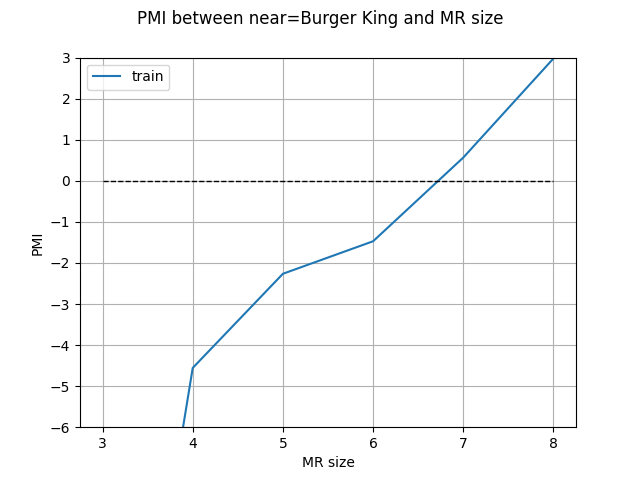
\includegraphics[scale=0.5]{nlg/nearbk.png}
\caption{PMI between \AV{near}{Burger King}~and \meaningrepresentation~size
on the E2E Challenge dataset. 0 on the $y$-axis indicates the two variables are independent.}
\label{fig:bkpmi}
\end{figure}


To demonstrate this, we trained a uni-directional GRU generation model on the
training corpus and then tried to generate an utterance for the following
\meaningrepresentation,
\begin{singlespace}
\[\mr = \left[\!\!\left[\begin{array}{l}\textsc{Inform}\\
        {\AV{name}{Alimentum}}  \\
        {\AV{near}{Burger King}}\\
        {\AV{area}{city centre}}\\
        {\AV{family\_friendly}{no}}\end{array}  \right]\!\!\right],\]
\end{singlespace}
\noindent using beam search. Notice that in this case $\setsize{\mr}=4$,
indicating that the occurrence of \textit{near=Burger King} is a relatively
novel situation given the training set.  We generated some beam search
candidates we show below, {\uline{underlining}} the phrases
that are not semantically correct given the \meaningrepresentation,

\begin{enumerate}
    \item Alimentum is located in the city centre {\uline{near the Express by Holiday Inn.}} It is not family-friendly.     
    \item Alimentum is located in the city centre {\uline{near the Yippee Noodle Bar.}} It is not family-friendly.
    \item Alimentum is located in the city centre {\uline{near the Raja Indian Cuisine.}} It is not family-friendly.
    \item Alimentum is not family-friendly. It is located in the city centre {\uline{near the Yippee Noodle Bar.}}
    \item The Alimentum is located in the city centre {\uline{near the Express by Holiday Inn.}} It is not family-friendly.
        %Alimentum is not family-friendly. It is located in the city centre near the Raja Indian Cuisine.\\\vspace{-1em}\\
        %Alimentum is located in the city centre near the Clare Hall. It is not family-friendly.\\\vspace{-1em}\\
        %Alimentum is located in the city centre near the crowne plaza hotel. It is not family-friendly.\\\vspace{-1em}\\
        %Alimentum is not family-friendly. It is located in the city centre near the express by holiday inn.\\\vspace{-1em}\\
        %The Alimentum is located in the city centre near the Yippee Noodle Bar. It is not family-friendly.\\\vspace{-1em}\\
        %Alimentum is not family-friendly. It is located in the city centre near the Clare Hall.\\\vspace{-1em}\\
        %The Alimentum is located in the city centre near the Raja Indian Cuisine. It is not family-friendly.\\\vspace{-1em}\\
        %In the city centre near the express by holiday inn is Alimentum. It is not family-friendly.\\\vspace{-1em}\\
        %Alimentum is located in the city centre near the city centre. It is not family-friendly.\\\vspace{-1em}\\
        %Alimentum is located in the city centre near the rice boat. It is not family-friendly.\\\vspace{-1em}\\
        %The Alimentum is not family-friendly. It is located in the city centre near the Yippee Noodle Bar.\\\vspace{-1em}\\
        %Alimentum is located in the city centre near the rainbow vegetarian café. It is not family-friendly.\\\vspace{-1em}\\
        %In the city centre near the Yippee Noodle Bar is the Alimentum. It is not family-friendly.\\\vspace{-1em}\\
        %In the city centre near the Yippee Noodle Bar is Alimentum. It is not family-friendly.\\\vspace{-1em}\\
        %
\end{enumerate}
Right away we are confronted by their homogeneity; utterances 1,2,3 and 5 have
the same syntactic structure, varying only in the phrase ``near X.'' Utterances
1 and 5 differ only by a single word (the initial article \textit{The} in 5).
Most importantly, none of them correctly specify that the Alimentum is near
Burger King. Even with a beam size of 128, the name ``Burger King'' is never
generated by the model!\footnote{A beam size of 128 would be impractical for
most applications. Beam sizes are typically from 4-10 in most works.}


\begin{figure}[p]
\centering
    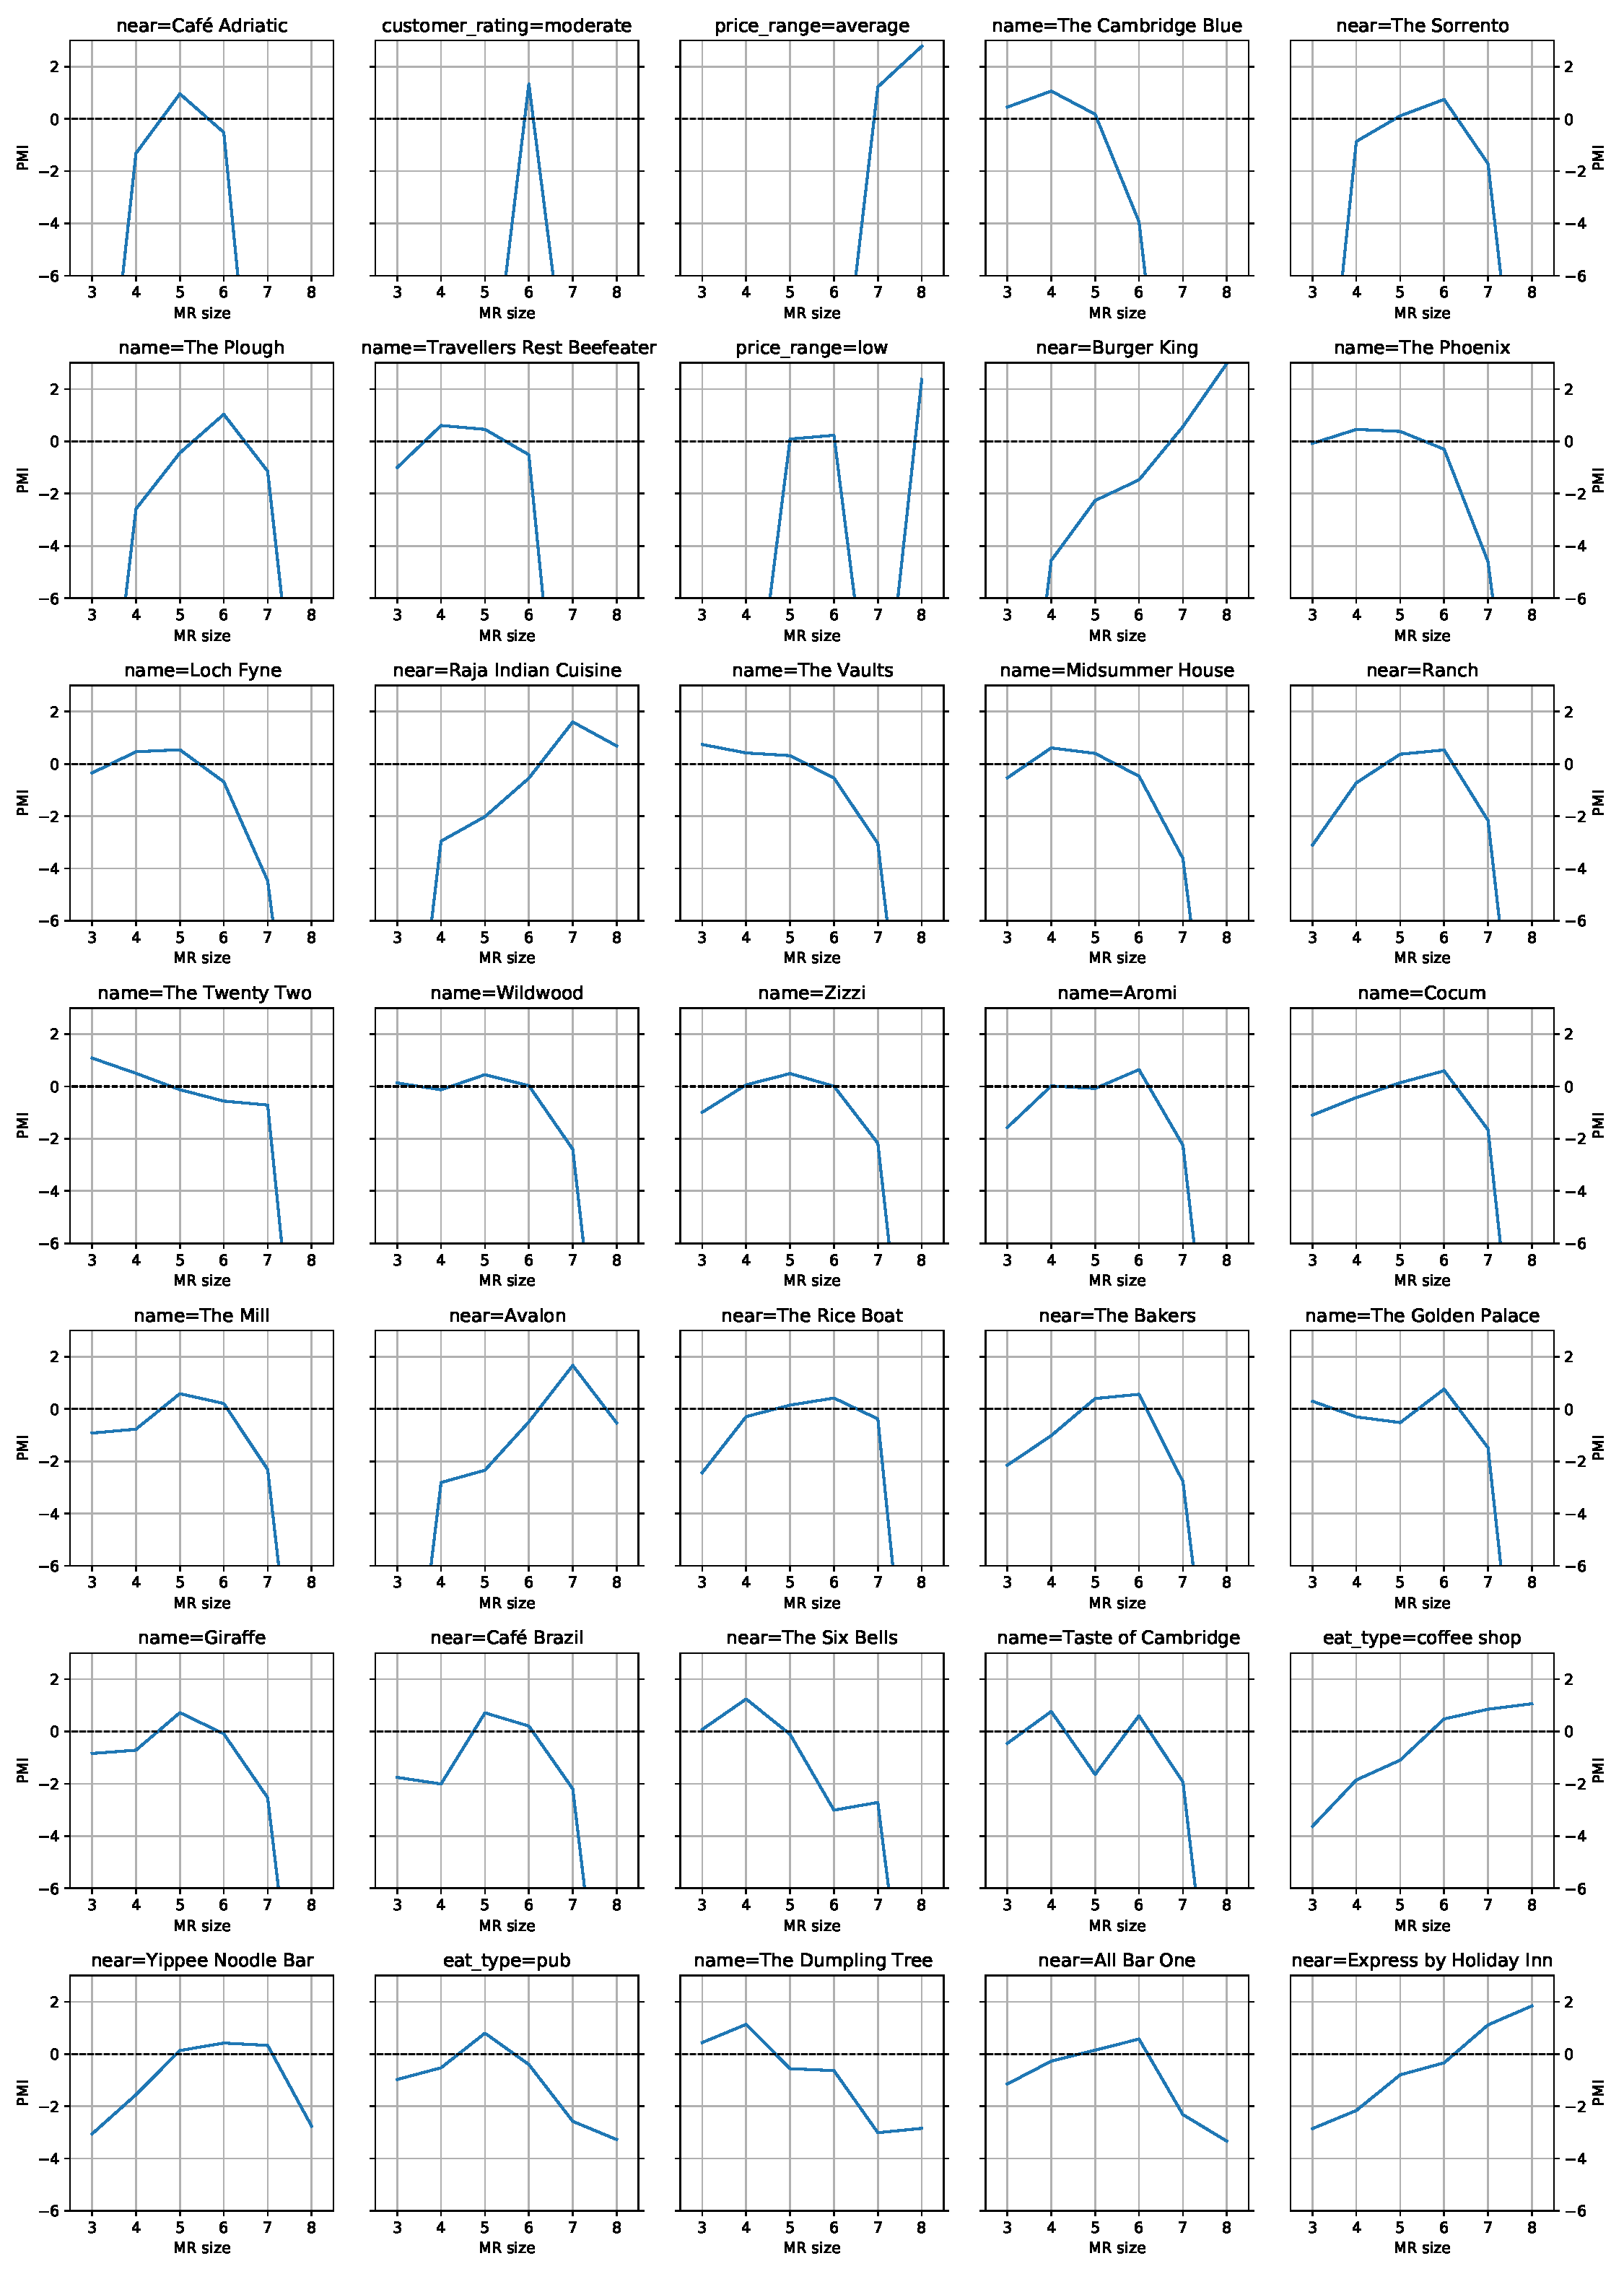
\includegraphics[width=0.9\textwidth]{nlg/trainpmis.pdf}
\caption{PMI between various \attributevalue s and \meaningrepresentation~size
on the E2E Challenge dataset. 0 on the $y$-axis indicates the two variables are independent.}
\label{fig:trainpmi}
\end{figure}


This is more frustrating because there are plenty of training examples where
even a coarse understanding of phrase structure would allow construction of a
correct utterance for this case.  For instance, we observe utterances
containing ``near Burger King'' like this,
\begin{quotation}
    \noindent \textit{The Eagle is a low rated coffee shop \textbf{near Burger King}
        and the riverside that is family friendly and is less than £20
    for Japanese food.}
\end{quotation}
while also seeing
\begin{quotation}
    \noindent \textit{Alimentum is located in the city centre \textbf{near Yippee Noodle Bar}. \textellipsis}
    % It serves expensive Italian food. It has an average customer rating.
\end{quotation}
where a correct utterance could be created by substituting ``Burger King''
in the latter instance, e.g., 
\begin{quotation}
    \noindent \textit{Alimentum is located in the city centre \textbf{near Burger King}.}
    % It serves expensive Italian food. It has an average customer rating.
\end{quotation}

Unfortunately, the GRU model does not learn to substitute the correct
prepositional phrase. Given that correct examples seem constructable from
constituent phrases, it suggests that a data-augmentation approach might help
to generate additional training examples that do not possess some of the
spurious correlations between \attributevalue s and input size.

Indeed, the compositional data-augmentation scheme proposed by
\citet{andreas2020} demonstrates  improved model systematicity.  Unfortunately,
a rule based system of recombination risks creating disfluencies in the
utterances that could potentially reduce the fluency of the learned model.
Additionally, the number of spurious associations in the dataset are numerous;
see \autoref{fig:trainpmi} for 35 of the total 79 \attributevalue~pairs for the
E2E dataset. They all have some spurious association with
\meaningrepresentation~size. And we haven't even explored other associations
that might exist (e.g. between two \attributevalue~pairs\footnote{One might
argue that it is OK for there to be correlations between the attribute-values,
e.g., maybe there are fewer family friendly restaurants in the city centre.
However, we often expect an NLG system to respond systematically -- given an
arbitrary set of attribute-values, the NLG component should realize them all
correctly, and under this constraint it is desirable that any particular
pairing of attribute values is independent in the NLG model.}).  In the
following subsections, we explore what an ideal data-augmentation policy might
look like and then give a practical implementation of it.

\subsection{An Idealized Data-Augmentation Protocol}
\label{sec:ideal}

We now introduce an idealized data-augmentation protocol and discuss some
potential pitfalls and bottlenecks before proposing our implementation of it.
Let $\corpus_\mrspace$ and $\corpus_\outSpace$ be the empirical distributions
(i.e. training dataset distributions) over the \meaningrepresentations~and
utterances respectively. The empirical distributions exhibit various dataset
creation/annotation artifacts. For example, we have that some attributes  are
correlated with length (i.e., $\corpus_\mrspace(a \in \mr, \setsize{\mr} = k)
\ne \corpus_\mrspace(a \in \mr)\corpus_\mrspace(\setsize{\mr} = k)$) or certain
attributes with each other (i.e., $\corpus_\mrspace(a_1, a_2 \in \mr) \ne
\corpus_\mrspace(a_1 \in \mr)\corpus_\mrspace(a_2\in \mr)$).

Ideally, we could construct novel \meaningrepresentation~examples such that
their distributions did not display these correlations. Let us assume we have
such a distribution, $\corpus_\mr^{-1}$, from which we can sample novel
utterances.  Given a sample $\corpus_\mr^{-1}$, we would then need a
conditional distribution $\daUttDist(\samplmr)$ from which to draw the
appropriate companion utterance $\samutttoks$ such that $\denotes{\samutttoks}
= \samplmr$ while the naturalness/grammaticality of $\samutttoks$ was
consistent with the empirical distribution, i.e. $S(\daUttDist) \approx
S(\corpus_\outSpace)$ where $S$ is a projection of utterances into a syntactic
space that is independent of the content.  Having these two distributions, we
could follow the simple data-augmentation protocol in \autoref{alg:idealda} to
obtain a more systematic language generation model $\gen_*$.

Coming up with a \meaningrepresentation~distribution, $\corpus_\mr^{-1}$, is
fairly straightforward.  For example we could just sample the size of the
\meaningrepresentation, $k$, uniformly at random, then sample the $k$
\attributes~uniformly at random without replacement. This would ensure that
attributes and \meaningrepresentation~size are independent and ensure that
\attributes~are not correlated with each other. To make up for the fact that
some \attributevalues~are over-represented in the training set, we could sample
values inversely proportional to their empirical frequency. This results in the
following data generation process for 
\begin{singlespace}\[
        \tilde{\mr}  = \left[\!\!\left[ 
                \begin{array}{c} 
                    \delta~~~~~~~ \\
                    \AV{$a_1$}{$v_1$} \\ \vdots \\ \AV{$a_k$}{$v_k$}  
                \end{array}  
\right]\!\!\right] \sim \corpus_\mr^{-1},\]\end{singlespace}
{
    \begin{minipage}{0.9\textwidth}
        \begin{singlespace}
            \noindent \textit{(1) Draw a dialogue act.}
            \[
                \delta \sim \operatorname{Uniform}(\left\{\delta_1, \delta_2,\ldots\right\}) 
            \]
            \noindent \textit{(2) Draw a \meaningrepresentation~size $k$.}
            \[
                k \sim \operatorname{Uniform}(\{k_{min}, \ldots, k_{max}\}) 
            \]
            \noindent \textit{(3) Sample $k$ attributes without replacement.}
            \[
            a_i  \sim \operatorname{Uniform}(\{name, \ldots, near, eat\_type\}\setminus\{a_1,\ldots,a_{i-1}\}) \quad \forall i: i \in  \{1,\ldots, k\}\]
            \noindent \textit{(4) Sample a value $v_i$ for each attribute $a_i$.}
            \[ v_i  \sim \operatorname{Categorical}\left(\operatorname{count}(v_1)^{-1}, \operatorname{count}(v_2)^{-1},\ldots\right)  \quad \forall i: i \in \{1,\ldots,k\}. \]
        \end{singlespace}
\end{minipage}}

\begin{algorithm}[t]
    $\augdata \gets \{\}$\\
    \While{$\setsize{\augdata} < \numSamples$}{
        $\tilde{\mr} \sim \corpus_\mr^{-1}$ \\
        $\boldsymbol{\tilde{\utttoks}} \sim \daUttDist(\boldsymbol{\tilde{\mr}})$\\
        %\If{ $\lnot \filter(\tilde{\mr}, \boldsymbol{\tilde{\utttoks}})$}{ $\augdata \gets \augdata \cup \{(\tilde{\mr}, \boldsymbol{\tilde{\utttoks}}) \}$ }
        $\augdata \gets \augdata \cup \{(\tilde{\mr}, \boldsymbol{\tilde{\utttoks}}) \}$
    }
    %    \KwResult{Salience judgements $\bsals = \left[ \bsal_1, \ldots, \bsal_\docSize\right]$}
    $\gen_* \gets \operatorname{Train}(\corpus \cup \augdata)$\\
    \KwResult{$\gen_*$}
    \caption{Idealized Data-Augmentation and Training}
    \label{alg:idealda}
\end{algorithm}~\\

Unfortunately, it is not clear how we implement utterance distribution
$\daUttDist(\samplmr)$ since if we had an utterance generation method that
could respond systematically to non-training data distributed
\meaningrepresentations, we wouldn't need to perform data augmentation in the
first place. As a starting point, we consider ways of generating samples from a
base model $\gen_0$  trained on the available training data, i.e.  $\gen_0 =
\operatorname{Train}(\corpus)$.

\subsection{Conditional Utterance Sampling for Data-Augmentation}

We cannot use $\gen_0$ with beam search as we saw previously; there are some
\meaningrepresentations~that $\gen_0$ won't be able to create utterances for
(as we saw with \textit{near=Burger King}). We could try a variant of ancestral
sampling, but it is difficult for ancestral sampling schemes to produce
extremely different outputs that break from spurious associations learned from
the training distribution without hurting fluency. 

The fundamental issue with ancestral sampling is that the randomness of the
model is located at the word selection stage. This means that in the middle of
generating a phrase it is possible for a disfluent word to be selected, which
can disrupt the current phrase but also destabilize subsequent generation steps
as the model tries to recover from the unusual selection.  Ideally, randomness
in a model would occur earlier in determining the ``topicality'' or
``aboutness'' (you might even say content selection) of the generated
utterance. 

Beyond the conditioning input $\ls(\mr)$, the content that is to be generated
is implicitly represented by inner hidden states of the model.  In
\citet{cho2016}, they argue that the hidden states, $\decHidState_i$, of the
\sequencetosequence~decoder lie on a manifold, as a requirement of learning the
next word prediction, i.e.  $\hat{\utttok} = \argmax_\utttok
\gen(\utttok|\utttoks_{1:i},\ls(\mr)) = \argmax_\utttok \left(\weight{o}
\decHidState_i + \bias{o}\right)_\utttok$ implies that $\hat{\utttok}$ must be
linearly separable from other words $\utttok^\prime \in \uttvocab$ along the
hidden state manifold. The implication is that moving about the manifold will
change the ``topicality'' of the distribution
$\gen(\utttok|\utttoks_{1:i},\ls(\mr))$.  They further suggest adding Gaussian
noise to $\decHidState_i$ as a way to obtain random samples from $\gen$, which
we refer to as \textit{noise-injection sampling}.  While \citet{cho2016} used
noise-injection sampling as a means to generate semantically correct but
syntactically diverse outputs, one of our contributions is to use this scheme
as a means to generate semantically divergent outputs (that maintain
grammaticality), for use as a data-augmentation tool.

\newtcbox{\stochbox}[1][]{colframe=blue, colback=blue!15, boxrule=0.1mm,
                       nobeforeafter, tcbox raise base, shrink tight, extrude
                       by=0.32mm, #1}
\newtcbox{\detbox}[1][]{colframe=red, colback=red!15, boxrule=0.1mm,
                       nobeforeafter, tcbox raise base, shrink tight, extrude
                       by=0.32mm, #1}


\renewcommand{\algorithmcfname}{Alg.}

\begin{figure}[t]
\begin{center}\small \detbox{Deterministic operation}~~~~\stochbox{Stochastic operation}\end{center}
\resizebox{\textwidth}{!}{%
\begin{minipage}{0.33\textwidth}
\small
\begin{singlespace}
\begin{algorithm}[H]
$\encHidState_{1:\mrSize} \gets \operatorname{enc}(\ls(\mr))$\\
$\predutttok_1 \gets \starttok$\\
$\predutttoks \gets \left[ \predutttok_1\right]$\\
$i \gets 1$\\
\While{$\predutttok_i \ne \stoptok$}{
$\decHidState_i \gets \operatorname{dec}(\predutttoks, \encHidState_{1:\mrSize})$\\
$\vphantom{\boldsymbol{\epsilon_i} \sim \operatorname{Normal}(\zeroEmb, \frac{\sigma}{i})}$\\
\detbox{$\predutttok_{i+1} \gets \argmax_\utttok \gen(\utttok|\decHidState_i)$}\\
$\predutttoks \gets \predutttoks \oplus \left[ \predutttok_{i+1}\right]$\\
$i \gets i + 1$\\
}
%$\gen_* \gets \operatorname{Train}(\corpus \cup \augdata)$\\
\KwResult{$\predutttoks$}
    \caption{\small Greedy Decoding}
%\label{alg:idealda}
\end{algorithm}
\end{singlespace}
\end{minipage}\begin{minipage}{0.33\textwidth}
\small
\begin{singlespace}
\begin{algorithm}[H]
$\encHidState_{1:\mrSize} \gets \operatorname{enc}(\ls(\mr))$\\
$\predutttok_1 \gets \starttok$\\
$\predutttoks \gets \left[ \predutttok_1\right]$\\
$i \gets 1$\\
\While{$\predutttok_i \ne \stoptok$}{
$\decHidState_i \gets \operatorname{dec}(\predutttoks, \encHidState_{1:\mrSize})$\\
$\vphantom{\boldsymbol{\epsilon_i} \sim \operatorname{Normal}(\zeroEmb, \frac{\sigma}{i})}$\\
\stochbox{$\predutttok_{i+1} \sim \vphantom{\argmax_\utttok}\gen(\cdot|\decHidState_i)$}\\
$\predutttoks \gets \predutttoks \oplus \left[ \predutttok_{i+1}\right]$\\
$i \gets i + 1$\\
}
%$\gen_* \gets \operatorname{Train}(\corpus \cup \augdata)$\\
\KwResult{$\predutttoks$}
\caption{\small Ancestral Sampling}
%\label{alg:idealda}
\end{algorithm}
\end{singlespace}
\end{minipage}\begin{minipage}{0.38\textwidth}
\small
\begin{singlespace}
\begin{algorithm}[H]
$\encHidState_{1:\mrSize} \gets \operatorname{enc}(\ls(\mr))$\\
$\predutttok_1 \gets \starttok$\\
$\predutttoks \gets \left[ \predutttok_1\right]$\\
$i \gets 1$\\
\While{$\predutttok_i \ne \stoptok$}{
$\decHidState_i \gets \operatorname{dec}(\predutttoks, \encHidState_{1:\mrSize})$\\
\stochbox{$\boldsymbol{\epsilon_i} \sim \operatorname{Normal}(\zeroEmb, \frac{\sigma}{i})$}\\
\detbox{$\predutttok_{i+1} \gets \argmax_\utttok \gen(\utttok|\decHidState_i + \boldsymbol{\epsilon_i})$}\\
$\predutttoks \gets \predutttoks \oplus \left[ \predutttok_{i+1}\right]$\\
$i \gets i + 1$\\
}
%$\gen_* \gets \operatorname{Train}(\corpus \cup \augdata)$\\
\KwResult{$\predutttoks$}
\caption{\small Noise Injection Sampling}
%\label{alg:idealda}
\end{algorithm}
\end{singlespace}
\end{minipage}
}
\caption{A comparison of greedy decoding, ancestral sampling, and noise injection sampling.}
\label{fig:noiseinj}

%?\begin{minipage}{0.3\textwidth}
%?\begin{singlespace}
%?\begin{algorithm}[H]
%?$\predutttok_1 \gets \starttok$\\
%?$i \gets 1$\\
%?\While{$\predutttok_i \ne \stoptok$}{
%?$\tilde{\mr} \sim \daMrDist$ \\
%?%\If{ $\lnot \filter(\tilde{\mr}, \boldsymbol{\tilde{\utttoks}})$}{ $\augdata \gets \augdata \cup \{(\tilde{\mr}, \boldsymbol{\tilde{\utttoks}}) \}$ }
%?$\augdata \gets \augdata \cup \{(\tilde{\mr}, \boldsymbol{\tilde{\utttoks}}) \}$
%?}
%?%    \KwResult{Salience judgements $\bsals = \left[ \bsal_1, \ldots, \bsal_\docSize\right]$}
%?$\gen_* \gets \operatorname{Train}(\corpus \cup \augdata)$\\
%?\KwResult{$\gen_*$}
%?    \caption{Noise-Injection Sampling}
%?\label{alg:idealda}
%?\end{algorithm}
%?\end{singlespace}
%?\end{minipage}
\end{figure}




\begin{figure}[t]
\small
\textbf{Ancestral Sampling}\\
\textit{\starttok~the eagle is a non family - friendly italian food establishment . \stoptok}\\
\textit{\starttok~the eagle is a italian food place and is not family - friendly . \stoptok}\\
\textit{\starttok~some italian food can be found at the eagle . \senttok~it 's not family - friendly . \stoptok}\\
\textit{\starttok~the eagle serves italian food . \senttok~it has a \unktok~\unktok~and is not family friendly . \stoptok}\\
\textit{\starttok~the eagle is a family friendly place for italian food . \stoptok}\\
~\\
\textbf{Top-K Sampling ($k=100$)}\\
\textit{\starttok~the eagle serves italian food . \senttok~it is not family - friendly . \stoptok}\\
\textit{\starttok~the eagle serves italian cuisine . \senttok~it is not family - friendly . \stoptok}\\
\textit{\starttok~the eagle has italian food and is not family - friendly \stoptok}\\
\textit{\starttok~the eagle is italian place . \senttok~it is not family - friendly . \stoptok}\\
\textit{\starttok~the eagle provides fast food . \senttok~it is not family - friendly . \stoptok}\\
~\\
\textbf{Nucleus Sampling ($p=0.95$)}\\
\textit{\starttok~the eagle serves italian food and is not family - friendly . \stoptok}\\
\textit{\starttok~the eagle is not family - friendly and serves italian food . \stoptok}\\
\textit{\starttok~the eagle is not family - friendly . \senttok~they serve italian food . \stoptok}\\
\textit{\starttok~italian food is served at the eagle . \senttok~not family - friendly . \stoptok}\\
\textit{\starttok~the eagle is a good place to eat italian food . \senttok~it is not family - friendly . \stoptok}\\
~\\
\textbf{Noise-Injection Sampling ($\sigma=2.0$)}\\
\textit{\starttok~the eagle in the city centre . \senttok~it is not family - friendly . \senttok~it is located near the burger king . \stoptok}\\
\textit{\starttok~the eagle serves italian food . \stoptok}\\
\textit{\starttok~the waterman is not family friendly and is located near burger king . \stoptok}\\
\textit{\starttok~the eagle is located near the burger king . \stoptok}\\
\textit{\starttok~the eagle is a non family - friendly italian food place . \stoptok}\\
\caption{Example samples taken after conditioning on the following  meaning representation: 
$\left[\!\!\left[\textsc{Inform};\quad    \AV{name}{The Eagle};\quad \AV{food}{Italian};\quad \AV{family\_friendly}{yes}\right]\!\!\right]$. }
\label{fig:examplesamples}
\end{figure}


We show the noise-injection sampling algorithm in \autoref{fig:noiseinj} along
with greedy decoding and ancestral sampling to emphasize the how the location
of the stochasticity moves from the next word selection
(\hyperref[fig:noiseinj]{Alg. \ref{alg:ancsam} line 8}) to a perturbation of
the hidden state (\hyperref[fig:noiseinj]{Alg.~\ref{alg:noiseinj} line 7}).
Note that in line 7 of the noise injection sampling algorithm, the standard
deviation of the normal distribution, $\frac{\sigma}{i}$, is scaled by the
decoder step $i$ and in the limit turns to zero, i.e. $\lim_{i \rightarrow
+\infty} \decHidState + \boldsymbol{\epsilon}_i = \decHidState$. The inuition
behind this scaling is that we add the most noise at the first steps of
decoding, which encourages the decoder to start from a topically novel region
of the hidden state manifold. As the decoding proceeds, the noise reduces along
with the chances of sending the decoder off the manifold and destabilizing the
decoding, and gradually we converge on the behavior of greedy decoding. 

We can understand noise-injection sampling as a compromise between greedy
decoding and ancestral sampling; rather than draw a sequence of utterance
tokens stochasticity, we instead draw a sequence of hidden state spaces.  Given
the sequence of hidden state spaces, the corresponding sequence of utterance
tokens is deterministically decided by the most likely next token given the
last hidden state. This next word selection strategy helps to avoid disfluent
continuations.

In \autoref{fig:examplesamples} we show examples of samples obtained with
noise-injection sampling as well as some ancestral sampling schemes.  We can
see that the ancestral sampling examples are not very diverse.  The
noise-injection sampling example, however, semantically diverges from the input
while maintaining fluency. It was even able to generate an utterance containing
the phrase ``near Burger King'' which is was practically impossible to generate
with beam search.

In \autoref{tab:sampprobs}, we show the probability of generating the example

\begin{center}
\textit{\starttok~the waterman is not family friendly and is located near burger king . \stoptok}\end{center}

\noindent under the various sampling schemes. In our present case, top-$k$ and
nucleus sampling have very similar distributions to the ancestral sampling
distribution ($\gen(\utttok_{i+1}|\decHidState_i)$). All three of these
techniques assign a very low probability to generating the example utterance,
and in the case of nucleus sampling, it only gives non-zero probability when
using a nucleus of 0.99 cumulative probability (i.e. $\nucleusVocab{i}{.99}$)!
In particular, noise-injection sampling puts much more probability mass on
generating relatively rare \attributevalue~realizations ($i=2$, ``waterman''
and $i=11$, ``burger''). This aspect of noise-injection sampling makes it very
attractive for data-augmentation as we can use it to create semantically novel
utterances that are not represented in the training dataset, while still
producing fluent outputs.

\begin{table}[p]
    \centering
    \begin{tabular}{c ccc ccc ccc ccc ccc c}
        \toprule
        $i$ & 1 & 2 & 3 & 4 &5 & 6 & 7\\
        $\utttok_{i+1}$ &  the  & waterman &is &not& family & friendly & and \\
        \midrule
        $\gen\left(\utttok_{i+1}|\decHidState_i; \topkVocab{i}{5}\right)$ & 0.874 & 0.004 & 0.380 & 0.397 & 0.915 & 0.147  & 0.338 \\
        $\gen\left(\utttok_{i+1}|\decHidState_i; \topkVocab{i}{25}\right)$ &
        0.792 & 0.004 & 0.344 & 0.371 & 0.877 & 0.147 & 0.327 \\
        $\gen\left(\utttok_{i+1}|\decHidState_i; \topkVocab{i}{50}\right)$ &
        0.778 & 0.004 & 0.339 & 0.366 & 0.872 & 0.147 & 0.326 \\
        $\gen\left(\utttok_{i+1}|\decHidState_i; \topkVocab{i}{75}\right)$ &
        0.772 & 0.004 & 0.338 & 0.364 & 0.870 & 0.147 & 0.326 \\
        $\gen\left(\utttok_{i+1}|\decHidState_i; \topkVocab{i}{100}\right)$ & 
        0.768 & 0.004 & 0.337 & 0.363 & 0.869 & 0.147 & 0.326 \\
        \midrule
        $\gen\left(\utttok_{i+1}|\decHidState_i; \nucleusVocab{i}{.95}\right)$     & 
        0.796 & 0.000 & 0.352 & 0.377 & 0.909 & 0.148 & 0.342 \\
        $\gen\left(\utttok_{i+1}|\decHidState_i; \nucleusVocab{i}{.96}\right)$ &
        0.789 & 0.000 & 0.349 & 0.374 & 0.898 & 0.148 & 0.338 \\
        $\gen\left(\utttok_{i+1}|\decHidState_i; \nucleusVocab{i}{.97}\right)$ &
        0.781 & 0.000 & 0.345 & 0.370 & 0.892 & 0.148 & 0.333 \\
        $\gen\left(\utttok_{i+1}|\decHidState_i; \nucleusVocab{i}{.98}\right)$ &
        0.773 & 0.000 & 0.342 & 0.367 & 0.882 & 0.148 & 0.332 \\ 
        $\gen\left(\utttok_{i+1}|\decHidState_i; \nucleusVocab{i}{.99}\right)$ &
        0.765 & 0.004 & 0.338 & 0.363 & 0.874 & 0.148 & 0.329 \\
        \midrule
        $\gen\left(\utttok_{i+1}|\decHidState_i\right)$ &0.758 & 0.004 & 0.335 & 0.359 & 0.865 & 0.147 & 0.326 \\
        $\gen\left(\utttok_{i+1}|\decHidState_i + \boldsymbol{\epsilon}_i\right)$ & 0.321 & 0.170 & 0.408 & 0.489 & 0.785 & 0.514 & 0.459 \\
        \bottomrule
    \end{tabular}

~\\~\\~\\~\\


    \begin{tabular}{c ccc ccc ccc ccc ccc}
        \toprule
        $i$             & 8 & 9 & 10 & 11 & 12 & 13 & 14 \\
        $\utttok_{i+1}$ &is& located &near& burger & king & . & \stoptok \\
        \midrule
        $\gen\left(\utttok_{i+1}|\decHidState_i; \topkVocab{i}{5}\right)$ & 0.111 & 0.147 & 0.168 & 0.000 & 0.954 & 0.931 & 0.810 \\
        $\gen\left(\utttok_{i+1}|\decHidState_i; \topkVocab{i}{25}\right)$ & 0.101 & 0.111 & 0.148 & 0.001 & 0.935 & 0.911 & 0.810 \\
        $\gen\left(\utttok_{i+1}|\decHidState_i; \topkVocab{i}{50}\right)$ & 0.100 & 0.105 & 0.146 & 0.001 & 0.930 & 0.910 & 0.810 \\
        $\gen\left(\utttok_{i+1}|\decHidState_i; \topkVocab{i}{75}\right)$ & 0.100 & 0.103 & 0.145 & 0.001 & 0.928 & 0.909 & 0.810 \\
        $\gen\left(\utttok_{i+1}|\decHidState_i; \topkVocab{i}{100}\right)$ & 0.100 & 0.102 & 0.144 & 0.001 & 0.926 & 0.909 & 0.810 \\
        \midrule
        $\gen\left(\utttok_{i+1}|\decHidState_i; \nucleusVocab{i}{.95}\right)$ & 0.104 & 0.103 & 0.150 & 0.000 & 0.964 & 0.950 & 0.810 \\
        $\gen\left(\utttok_{i+1}|\decHidState_i; \nucleusVocab{i}{.96}\right)$ & 0.103 & 0.102 & 0.149 & 0.000 & 0.954 & 0.939 & 0.810 \\
        $\gen\left(\utttok_{i+1}|\decHidState_i; \nucleusVocab{i}{.97}\right)$
     & 0.102 & 0.101 & 0.148 & 0.000 & 0.947 & 0.931 & 0.810 \\
        $\gen\left(\utttok_{i+1}|\decHidState_i; \nucleusVocab{i}{.98}\right)$   
     & 0.101 & 0.100 & 0.146 & 0.000 & 0.937 & 0.924 & 0.810 \\
        $\gen\left(\utttok_{i+1}|\decHidState_i; \nucleusVocab{i}{.99}\right)$
     & 0.100 & 0.099 & 0.145 & 0.001 & 0.928 & 0.917 & 0.810 \\
 \midrule
        $\gen\left(\utttok_{i+1}|\decHidState_i\right)$ & 0.099 & 0.098 & 0.143 &0.001 & 0.919 & 0.908 & 0.810\\
        $\gen\left(\utttok_{i+1}|\decHidState_i + \boldsymbol{\epsilon}_i\right)$ & 0.562 & 0.440 & 0.731 &0.599 & 0.972 & 0.903 & 0.984 \\
 \bottomrule
    \end{tabular}

    \caption{Word selection probabilities when using ancestral sampling,
        top-$k$ sampling (for $k \in \{5,25,50,75,100\}$), 
    nucleus samplling (for $\nucleusthr \in \{0.95, 0.96, 0.97, 0.98, 0.99\}$), and noise-injection sampling ($\sigma = 2.0$).}
    \label{tab:sampprobs}
\end{table}




\subsection{A Practical Data-Augmentation Protocol}
\label{sec:daprotos}


\newtcbox{\truttbox}[1][]{colframe=green, colback=green!15, boxrule=0.1mm,
                       nobeforeafter, tcbox raise base, shrink tight, extrude
                       by=0.32mm, #1}
\newtcbox{\mrdistbox}[1][]{colframe=orange, colback=orange!15, boxrule=0.1mm,
                       nobeforeafter, tcbox raise base, shrink tight, extrude
                       by=0.32mm, #1}

\newtcbox{\ninjbox}[1][]{colframe=purple, colback=purple!15, boxrule=0.1mm,
                       nobeforeafter, tcbox raise base, shrink tight, extrude
                       by=0.32mm, #1}
\newtcbox{\correctbox}[1][]{colframe=blue, colback=blue!15, boxrule=0.1mm,
                       nobeforeafter, tcbox raise base, shrink tight, extrude
                       by=0.32mm, #1}
\newtcbox{\filterbox}[1][]{colframe=cyan, colback=cyan!15, boxrule=0.1mm,
                       nobeforeafter, tcbox raise base, shrink tight, extrude
                       by=0.32mm, #1}

\newtcbox{\returnbox}[1][]{colframe=violet, colback=violet!15, boxrule=0.1mm,
                       nobeforeafter, tcbox raise base, shrink tight, extrude
                       by=0.32mm, #1}

%\begin{figure}[t]
%\begin{singlespace}
\begin{algorithm}[Ht]
\truttbox{$\gen_0 \gets \operatorname{Train}_\utttoks\left(\corpus\right)$} \\
\truttbox{$\dmodel \gets \operatorname{Train}_\mr\left(\corpus\right)$} \\
$\augdata \gets \left\{ \right\}$\\
\While{$\setsize{\augdata} < \numSamples$}{
\mrdistbox{$\samplmr \sim \pdaMrDist$}\\
\ninjbox{$\pdaCandUtts_{200}\gets \left\{ \pdaCandUtt \sim 
            \gen_0\left(\cdot|\ls(\samplmr), \pdaCandEps\right) 
            \quad \forall i : i \in \{1,\ldots, 200\} \right\} $}\label{lst:pdacand}\\

            \ninjbox{$\pdaCandUtts_{20} \gets \operatorname{Top}_{20}\left(
                \pdaCandUtts_{200}, \lambda\utttoks : 
        \frac{\log \gen_0\left(\utttoks|\ls(\samplmr),\boldsymbol{\epsilon} \right)}{\setsize{\utttoks}}\right)$}\label{lst:pdacandselect}\\
%\ninjbox{$\predutttoks \gets
%    \argmax_{\pdaCandUtt \in \pdaCandUtts} 
%    \frac{\log \gen_0\left(\pdaCandUtt|\ls(\samplmr),\pdaCandEps \right)}{\setsize{\pdaCandUtt}}$}\label{lst:pdacandselect}\\
        \For{$\predutttoks \in \pdaCandUtts_{20}$}{
\correctbox{$\pdaPredMr \gets \dmodel\left(\predutttoks\right)$}\\
\If{\filterbox{$\lnot \operatorname{Filter}\left(\pdaPredMr, \predutttoks\right)$}}{
    $\augdata \gets \augdata \cup \left\{ \left(\pdaPredMr, \predutttoks\right) \right\}$
}
~\\
}}
\returnbox{$\auggen \gets \operatorname{Train}_\utttoks(\corpus \cup \augdata)$}\\
\KwResult{$\auggen$}
    \caption{Data Augmentation with Noise-Injection Sampling and Self-Training }
\label{fig:practda}
%\label{alg:idealda}
\end{algorithm}
%\end{singlespace}
%\caption{A comparison of greedy decoding, ancestral sampling, and noise injection sampling.}
%\end{figure}


Because of its ability to generate semantically divergent and novel outputs
while maintaining fluency, we adopt this noise-injection sampling as our method
of sampling utterances, $\daUttDist$, for data-augmentation. We show our actual
data-augmentation scheme in \autoref{fig:practda} and now walk through some of
the implementation details.

%\paragraph{\truttbox{Train base generator $\gen_0$ and
%\meaningrepresentation~parser $\dmodel$.}} 
\paragraph{{Train base generator $\gen_0$ and
\meaningrepresentation~parser $\dmodel$.}} 
The algorithm begins by training the
base generator (i.e., na{\"i}ve \sequencetosequence~model) and
\meaningrepresentation~parser $\dmodel$.  Both models are trained on the same
data, with the only real change to the $\operatorname{Train}$ sub-routine being
which part of a training example is the output and which is the input.
Alternatively, $\dmodel$ can also be implemented using regular-expression-based
rules. We defer detailed explanation of $\dmodel$ until the experiments; it
suffices to understand $\dmodel$ as a mapping from utterances to
\meaningrepresentations.

%\paragraph{\mrdistbox{Sampling a \meaningrepresentation, $\samplmr$}}
\paragraph{{Sampling a \meaningrepresentation, $\samplmr$}}
We use the meaning representation sampling scheme described in
\autoref{sec:ideal} to implement the distribution $\corpus_\mr^{-1}$. 

%\paragraph{\ninjbox{Generating a novel utterance from $\basegen$ with
%noise-injection sampling.}} 
\paragraph{{Generating a novel utterance from $\basegen$ with
noise-injection sampling.}} 
In \autoref{lst:pdacand} we take $200$
noise-injection samples from $\basegen$ to construct a candidate set of
utterances, $\pdaCandUtts_{200}$.  We use $\sigma=2.0$ after manually
experimenting with a range of values from 0.1-3.0 since it gave reasonably
fluent outputs while also generating semantically divergent outputs..  phrases
with no realized attributes.  From these we use only the top 20 utterances,
$\pdaCandUtts_{20}$ by average log-likelihood,
$\frac{\log\gen(\pdaCandUtt|\ls(\samplmr),
\boldsymbol{\epsilon}^{(i)})}{\setsize{\pdaCandUtt}}$
(\autoref{lst:pdacandselect}).  We do this selection step so as to be extra
cautious and avoid adding any potentially disfluent utterances to $\augdata$.
    
%\paragraph{\correctbox{Predict \meaningrepresentation~$\pdaPredMr$ from
%$\predutttoks$.}} 
\paragraph{{Predict \meaningrepresentation~$\pdaPredMr$ from
$\predutttoks$.}} 
Because the noise-injection sampling produces highly
semantically divergent utterances, it is unlikely that $\denotes{\predutttoks }
= \samplmr$. Instead we use the \meaningrepresentation~parser, $\dmodel$, to
recover the most likely \meaningrepresentation, $\pdaPredMr =
\dmodel\left(\predutttoks\right)$.  More details about $\dmodel$ will be
provided in \autoref{sec:mrparsermodels}.

%\paragraph{\filterbox{Check synthetic datapoint $(\pdaPredMr,\predutttoks)$.}}
\paragraph{{Check synthetic datapoint $(\pdaPredMr,\predutttoks)$.}}
We do one last quality check on the synthetic example
$(\pdaPredMr,\predutttoks)$ before adding it to the augmented dataset,
$\augdata$. We make sure that the probability of $\pdaPredMr$ under $\dmodel$
is above 0.5 when using a model-based \meaningrepresentation~parser. When using
a rule-based \meaningrepresentation~parser, we check to make sure that there
are no repeated \attributevalue-pairs in $\predutttoks$, e.g., ``Aromi is a
coffee shop and it is a coffee shop,'' by discarding any utterances that
trigger multiple rules for any attribute.  Meaning representation/utterances
that have been previously generated are also discarded. If the
\meaningrepresentation/utterance pair passes these final quality checks, we add
it to $\augdata$.

%\paragraph{\returnbox{Train an augmented generator $\auggen$ on $\corpus \cup
%\augdata$.}} 
\paragraph{{Train an augmented generator $\auggen$ on $\corpus \cup
\augdata$.}} 
After generating a synthetic dataset, $\augdata$, we train a new
generation model, $\auggen$, on the union of the original training data and the
newly generated synthetic data. We refer to this model as the augmented
generator and, as we will show empirically, the augmented generator is more
faithful than the base generator, $\gen_0$.  We call this process self-training
because $\auggen$ and $\gen_0$ share the same architecture, and $\auggen$ is
trained on data produced by $\gen_0$. In theory, we could repeat this process
similar to iterative back-translation \citep{hoang2018}, using $\gen_0$ to
produce a $\gen_1$ which could then produce a $\gen_2$ and so on. However, we
did not experiment with this because we found that $\auggen$ improved in
faithfulness significantly over $\gen_0$ after one pass through
\autoref{fig:practda}.

\subsection{Datasets}

\begin{table}
\centering
\begin{tabular}{ccc ccc}
\toprule
Dataset & Train & Valid & Test & Unique Dialogue Acts & Unique Attribute Values \\
\midrule
E2E Chal. & 42,061 & 4,672 & 4,693 & 1 & 8 \\
Laptops & 15,888 & 5,298 & 5,297 & 14 & 19\\
TVs & \phantom{0}8,442 & 2,814 & 2,812 & 14 & 15\\
\bottomrule
\end{tabular}
\caption{Dataset statistics for noise-injection and self-training 
experiments.}
\label{tab:fgds}
\end{table}


We experimentally validate the noise-injection sampling and self-training
data-augmentation scheme on three recent dialogue generation datasets, the E2E
Challenge dataset~\citep{novikova2017} and the Laptops and TVs datasets
\citep{wen2016}.  Each dataset consists of \meaningrepresentations~paired with
one or more reference utterances.  All attribute values come from a closed
vocabulary.

The three datasets also represent different training size conditions; with the
E2E Challenge dataset representing the ``large data'' training condition and
the Laptops and TVs dataset representing ``small data'' conditions. See
\autoref{tab:fgds} for dataset size statistics.  The E2E Challenge dataset has
only one dialogue act, \textsc{Inform}, and its training
\meaningrepresentations~contain three to eight unique attributes.  The Laptops
and TVs datasets contain a more diverse set of \meaningrepresentation/utterance
pairs. There are 14 unique dialogue acts.  The number of minimum and maximum
\attributes~varies according to the dialogue act. See \autoref{tab:fgdas} for a
list of the unique dialogue acts and attributes for the three training sets. 

\begin{table}
\centering
\begin{tabular}{llll}
\toprule
Dataset & Dialog Acts & \multicolumn{2}{c}{Attributes} \\
\midrule
 \multirow{8}{*}{E2E Challenge} & \textsc{Inform} & name \\
 & & near \\
 & & eat\_type \\
 & & food \\
 & & area \\
 & & price\_range \\
 & & customer\_rating \\
 & & family\_friendly \\
\midrule
\multirow{14}{*}{Laptops} & \textsc{Inform} & family & weight\\
& \textsc{InformOnlyMatch} & price\_range & platform\\
& \textsc{InformOnMatch} & battery\_rating & memory\\
& \textsc{InformAll} & drive\_range & drive \\ 
& \textsc{InformCount} & weight\_range & processor \\
& \textsc{InformNoInfo} & is\_for\_business\_computing\\
& \textsc{Recommend} &name\\ 
& \textsc{Compare}& type \\
& \textsc{Select}& price\\
& \textsc{Suggest}& warranty\\
& \textsc{Confirm} & battery\\ 
& \textsc{Request}&design\\
& \textsc{RequestMore} &dimension \\
& \textsc{Goodbye} & utility\\
\midrule
 \multirow{14}{*}{TVs} & \textsc{Inform} & family & audio \\
& \textsc{InformOnlyMatch} & price\_range \\
& \textsc{InformOnMatch} & screen\_size\_range \\
& \textsc{InformAll} & eco-rating\\ 
& \textsc{InformCount}& hdmi-port\\
& \textsc{InformNoInfo}& has\_usb-port\\
& \textsc{Recommend} & name \\ 
& \textsc{Compare} & type \\
& \textsc{Select} &price\\
& \textsc{Suggest} & resolution\\
& \textsc{Confirm} & power\_consumption\\ 
& \textsc{Request} & accessories\\
& \textsc{RequestMore}& color \\
& \textsc{Goodbye} & screen\_size\\
\bottomrule
\end{tabular}
\caption{The dialogue acts and attributes for the E2E Challenge, Laptops, and TVs datasets.}
\label{tab:fgdas}
\end{table}


\paragraph{Delexicalization}
Prior work using neural \naturallanguagegeneration~models often relies on
delexicalization, that is, replacing realizations of named-entity or numeric
values in an utterance with a placeholder token, in order to alleviate data
sparsity issues and yield better generalization when a generating utterances
about named-entities not seen in the training dataset. For example, on the E2E
Challenge dataset, the \Atr{name}~and \Atr{near}~attributes are often
delexicalized because they are proper names of establishments that are simple
to find and replace in the utterance.  When delexicalizing the \Atr{name}~and
\Atr{near}~attributes, the fully lexicalized utterance 

\begin{center}\noindent~~~~\textit{Near The Six Bells is a venue that is children
friendly named The Golden Curry.}\end{center}

\noindent can be delexicalized as

\begin{center}\noindent ~~~~\textit{Near <<near>> is a venue that is children
friendly named <<name>>.}\end{center}

\noindent Delexicalized utterances can be re-lexicalized as a post-processing
step, where the placeholder token is replaced with the correct value text.

On the E2E Challenge dataset, we experiment with delexicalization of the
\textit{Name} and \textit{Near} attributes since they have a relatively large
vocabulary of valid slot fillers, some of which are only seen  infrequently in
the training data; it can be difficult for fully lexicalized models to produce
some of the rarer location names for these attributes.  However, since
delexicalization might be difficult or impossible in other domains, we
implement both delexicalized and lexicalized versions of the generation models
on the E2E dataset to more fully evaluate the self-training method.
   
The evaluation script for the Laptops and TVs datasets uses delexicalization to
evaluate attribute realization error, and so we use it here to be consistent
with prior work, delexicalizing all possible attributes.

While delexicalization effectively solves some problems in faithful generation
(e.g., the difficulty in generating the phrase \textit{``near Burger King''}),
it is difficult to apply to attributes that are not realized by a small
vocabulary of names or phrases. Even in those cases it introduces extra
complexity if the surrounding context will depend on the particular value in
any way (e.g., \textit{``near an <<name>>''} would not be grammatical if
replacing the \textit{<<name>>} placeholder with \textit{``Burger King''}).

\subsection{Text Generation Models}
\label{sec:fgtgm}

We use a two-layer, unidirectional GRU architecture with Bahdanau style
attention for our \sequencetosequence~\meaningrepresentation-to-text model. We
set $\embDim = \hidDim = \encDim = \decDim = 512$, that is, we use
512-dimensional embedding and hidden states as described in
\autoref{sec:nlggru}.  We fit model parameters, $\params$, by minimizing the
negative log-likelihood of the training set, $\corpus$, i.e.
\[\mathcal{L}(\params) = - \sum_{(\mr, \utttoks) \in \corpus  }  \log
\gen\left(\utttoks|\ls(\mr);\params\right).\]

Our choice of linearization strategy, $\ls$, differs slightly for the E2E
Challenge and ViGGO corpora. For the former, we arbitrarily and consistently
order the eight attribues, explicitly representing absent \attributevalues~with
a \textit{N/A} token.\footnote{In our initial experiments, including absent
attributes in the input this way performed slightly better than omitting them.}
For example, for the \meaningrepresentation
\begin{singlespace}
    \[\mr = \left[\!\!\left[ \begin{array}{l}
    \textsc{Inform}\\
    {\AV{name}{The Mill}}\\
    {\AV{near}{Avalon}}\\
    {\AV{food}{Italian}}  \end{array} \right]\!\!\right],\]
\end{singlespace}
\noindent we would have the following linearization,\begin{singlespace}
\[ \ls(\mr) = \left[\begin{array}{l} \starttok,\\ \textit{eat\_type=N/A},\\ \textit{near=Avalon},\\ \textit{area=N/A}, \\ \textit{family\_friendly=N/A},\\ \textit{customer\_rating=N/A}, \\\textit{price\_range=N/A},\\ \textit{food=Italian},\\ \textit{name=The Mill}\\ \stoptok \end{array}\right].\] \end{singlespace}
\noindent We omit the dialogue act since the E2E Challenge dataset only has one, \textsc{Inform}. When
    using the delexicalized model variant, we omit the name attribute since
    it is always present, and only indicate that the near attribute is present
    with a placeholder
    token, yielding \begin{singlespace}
\[ \ls(\mr) = \left[\begin{array}{l} \starttok,\\ \textit{eat\_type=N/A},\\ \textit{near=<<present>>},\\ \textit{area=N/A}, \\ \textit{family\_friendly=N/A},\\ \textit{customer\_rating=N/A}, \\\textit{price\_range=N/A},\\ \textit{food=Italian},\\ \stoptok \end{array}\right].\] \end{singlespace}

For the Laptops and TVs corpus, we similarly determine an arbitrary ordering
but omit any absent attribute-values since there are too many to represent all
of them explicitly. Additionally, since there are multiple dialogue acts we
prepend a token representing the dialogue act to the start of the sequence. As
an example, for the following \meaningrepresentation\\[-15pt]
\begin{singlespace}
   \[ \mr =\left[\!\!\left[ \begin{array}{l} 
    \textsc{InformCount} \\
    {\AV{count}{40}}\\
    {\AV{family}{don't care}}\\
    {\AV{battery\_rating}{excellent}}\end{array} \right]\!\!\right] \]
\end{singlespace}~\\
\noindent we would have the following linearization,
\[
    \ls(\mr) = \left[\starttok, \textit{inform\_count}, \textit{count=<<NUM>>}, \textit{family=don't care}, \textit{battery\_rating=excellent}, \stoptok\right].  
\]

When generating utterances for evaluation (i.e. not for use in noise-injection
sampling) we use either greedy decoding or beam decoding with a beam size of
eight.  The beam search terminates after eight candidates have been generated;
the candidates are reranked by average token log-likelihood, $\frac{\log
\gen\left(\utttoks|\ls(\mr)\right)}{\setsize{\utttoks}}$. In these experiments,
we \textbf{do not} use a discriminative reranker to ensure the faithfulness of
the selected beam candidate. 

\subsection{\MeaningRepresentation~Parsing Models}
\label{sec:mrparsermodels}

Given a novel utterance $\predutttoks$~sampled from $\basegen$, we need to
reliably parse the implied meaning representation  $\pdaPredMr =
\dmodel(\predutttoks)$, where $\dmodel$~is our parsing model. We have two
things going for us in our experimental setting. First, even with
noise-injection sampling, model outputs are fairly patterned, reducing the
variability of the utterances we need to parse in practice; a
\meaningrepresentation~parser on real human data would need to be much more
robust.

Second, the \meaningrepresentation~in this study are flat lists of attributes
that are somewhat independent of each other.  We only need to detect the
presence of each attribute and its value.  For the Laptops and TVs datasets we
also need to recover the dialog act but these also are signaled by a fairly
limited repertoire of cues, e.g. ``we recommend.'' Given this, we experiment
with both hand crafted regular expression rules and learned classifiers to
predict the value of an attribute if present or that it is missing. 

\paragraph{Rule-based parser (\ruledmodel)} We design hand-crafted regular
expression based rules to match for the presence of key phrases for each of the
attributes and dialouge acts in the datasets while also checking to make sure
that there is only one match per attribute.

To construct the rules, we look through both the training data references as
well as the generation model outputs as this is what the rules will be
operating on in practice. For each lexicalized attribute (and dialogue act) we
develop a list of regular expressions such as,\[
\texttt{/is (family|kid|child) friendly/} \Rightarrow \AV{family\_friendly}{yes}.\]
For the delexicalized attributes, we simply check for the presence of the
placeholder token. 

We design these rules to be high precision, as it is safer to miss out on 
more obscure varieties of utterance to avoid adding incorrectly parsed data 
points.
However,  in many cases the rules are also high recall as well. 
The average F-score on the E2E validation set is 0.93.

\paragraph{Classifier-based parser (\learndmodel)} 

It is perhaps too optimistic to believe we can construct reasonable rules in
all cases. Rule creation quickly becomes tedious and for more complex
\meaningrepresentations, this would become a bottleneck. To address these
concerns, we also study the feasibility of using learned classifiers to predict
the presence and value of the attributes. For each attribute in the E2E
dataset, we trained a separate convolutional neural network classifier to
predict the correct attribute value (or \textit{n/a} if the attribute is not
present) from an utterance.

The architecture largely follows that of \citet{kim2014convolutional}.  Let
$\parEmbs \in \reals^{\setsize{\uttvocab} \times \parEmbsDims}$ be an embedding
matrix for the utterance token vocabulary, $\parEmbs$, with each token $\utttok
\in \uttvocab$ associated with a row in $\parEmbs$, which we indicate with
$\parEmbs_\utttok \in \reals^{\parEmbsDims}$.  For each attribute $\attr$, the
set of possible values (including \textit{n/a}) is denoted $\attrvocab$.

Given an utterance $\utttoks = \left[\utttok_1,\ldots,\utttok_\uttSize\right],$
we first embed the utterance tokens to obtain a sequence of word embeddings, \[
\parEmb_1, \ldots, \parEmb_\uttSize = \parEmbs_{\utttok_1}, \ldots,
\parEmbs_{\utttok_\uttSize}. \]

We then apply a series of unigram, bigram, and trigram convolutional filters
(i.e., convolutional feature widths $\parkwidth$ of 1, 2, and 3 respectively)
each with $\parFtrDims$ output features, which are computed as,
\begin{align*} \parFeat_{k,i} & = 
    \max_{j \in \convRange{\parkwidth}{\uttSize} } 
    \relu\left(\convbias{k,i} + \convweight{k,i} \cdot
\left[\begin{array}{c} \parEmb_j \\ \parEmb_{j+1}\\\vdots \\\parEmb_{j+k-1} \end{array}  \right]\right)  \quad \forall k,i: \begin{array}{l} k \in \{1,2,3\}, \\[-1em] i \in \{1,\ldots, \parFtrDims\} \end{array}
\end{align*}
where $\convbias{k,i} \in \reals$ and $\convweight{k,i} \in
\reals^{\parkwidth\parEmbsDims}$ are learned parameters and we use the same
zero-padded convolution described in \autoref{sec:sentconvenc} with $\parEmb_i
= \zeroEmb$ for $i < 1$ and $i > \uttSize$.  The individual convolutional
features are collected in a hidden state encoding of the utterance, $\parHid
\in \reals^{\parkwidth \parFtrDims}$, with
\[
\parHid = \left[\parFeat_{1,1},\ldots,\parFeat_{1,\parFtrDims},\parFeat_{2,1},\ldots,\parFeat_{2,\parFtrDims}, \parFeat_{3,1}, \ldots, \parFeat_{3,\parFtrDims}\right].
\] 
The hidden state is then fed through a two layer \feedforward~network to
compute the probability of a particular attribute value,
\[    
\dmodel_\attr\left(\aval|\utttoks\right)   = \softmax\left(\cweight{\attr,2} \left( \cweight{\attr,1} \parHid + \cbias{\attr,1}\right)   + \cbias{\attr,2} \right)_\aval
\]
where $\cweight{\attr,1} \in \reals^{\parEmbsDims \times
\parkwidth\parEmbsDims}$, $\cbias{\attr,1} \in \reals^{\parEmbsDims}$,
$\cweight{\attr,2} \in \reals^{\setsize{\attrvocab} \times \parEmbsDims}$, and
$\cbias{\attr,2} \in \reals^{\setsize{\attrvocab}}$ are learned parameters. If
$\mr$ contains a $\mrSize$ \attributevalue~pairs,
$\attr_1=\aval_1,\ldots,\attr_\mrSize=\aval_\mrSize$, the probability of $\mr$
under the parsing model is $\dmodel(\mr|\utttoks) = \prod_{i=1}^\mrSize
\dmodel_{\attr_i}\left(\aval_i|\utttoks \right)$.

Each attribute classifier has distinct parameters and is trained on the
training set but minimizing the negative log-likelihood,
\[\mathcal{L}(\dparams) = -\sum_{(\attr=\aval, \utttoks) \in \corpus} \log
\dmodel_\attr(\aval| \utttoks;\dparams),  \] using minibatch stochastic
gradient descent on the training set, $\corpus$.

During training we apply dropout (with drop rate of 0.25) to the embedding
layer, convolutional filter outputs, and hidden layers. We train for 30 epochs
with gradient descent using  a learning rate of 0.25 and weight decay penalty
of 0.0001, using validation set F1 as our model selection criterion.  The
average E2E validation F-score is 0.94.

\subsection{Experiments}
\subsubsection{E2E Challenge}
We train base generators $\basegen$~on the original training data $\corpus$,
with and without delexicalizing the \Atr{name} and \Atr{near} attributes.  We
train for 500 epochs with gradient descent. We use a batch size of 128, with a
learning rate of 0.25, weight decay penalty of 0.0001, and a dropout
probability of 0.25.  We select the best model iteration using validation set
\bleu~score.\footnote{We use the official shared task script to compute
automatic quality metrics on the E2E dataset.}

Using the self-training method outlined in \autoref{sec:daprotos}, we create
augmented datasets using either $\ruledmodel$~or $\learndmodel$, which we refer
to as $\augdata_{\ruledmodel}$ and $\augdata_{\learndmodel}$ respectively We
only use the model parser, $\learndmodel$, in the delexicalized setting.  We
repeat the while loop in the data-augmentation algorithm 25,000 times for each
valid MR size $3,\ldots,8$, yielding 1,591,788 additional samples for the
lexicalized $\gen_0/\ruledmodel$ pairing, and 501,909 for $\gen_0/\ruledmodel$
and 384,436 for $\gen_0/\learndmodel$~delexicalized pairings.\footnote{The
number of additional examples generated by the delexicalized approaches is an
order of magnitude smaller than the lexicalized case because we discard
duplicate generated utterances.  With delexicalization, duplicates are more
frequently generated by the model.}

For both $\corpus \cup \augdata_{\ruledmodel}$ and $\corpus \cup
\augdata_{\learndmodel}$ we train new generators \auggen~using the same
training setting as above (although we terminate training after 50 epochs
because the models converge much faster with the additional data).  We report
\textsc{Bleu}, \textsc{Rouge-L}, and \textsc{Meteor} on the E2E Challenge test
set, using the official shared-task evaluation script.  We show results for
both greedy decoding and beam decoding with beam size 8 under $\basegen$~and
\auggen~models. We compare our models to the best sequence-to-sequence model,
Slug \citep{juraska2018}, the best grammar-rule based model, DANGNT
\citep{nguyen2018}, and the best template based model, TUDA
\citep{puzikov2018}, as determined during the shared task evaluation
\citep{dusek2019}.

\subsubsection{Laptops and TVs}

We perform similar experiments on the Laptops and TVs datasets.  We train a
separate $\basegen$~model for each dataset for 300 epochs with a learning rate
of 0.1 for Laptops and 0.25 for TVs. The weight decay penalty is 0.0001 and
dropout probability is 0.25. Best model iteration is determined by validation
set \textsc{Bleu} score. As in the E2E experiments, we create an augmented
dataset for both the Laptops and TVs dataset using the method outlined in
\autoref{sec:daprotos}. We then train new generators $\auggen$~on the union of
original training data and the augmented dataset.

We repeat the while loop in the noise-injection sampling algorithm 25,000 times
for each dialogue act and legal dialogue act size.\footnote{A number of
attributes $S$ is ``legal'' if we observe a training instance with that
dialogue act instance with $S$  attributes in the original training data.} We
obtain 373,468 and 33,478 additional samples for the Laptops and TVs datasets
respectively.

We automatically evaluate our models using the evaluation script of
\citep{wen2016}, which computes \textsc{Bleu} scores, as well as slot alignment
error rate (since this dataset is almost fully delexicalized, it simply checks
for the presence of the correct attribute placeholders according to the MR). We
compare again to the Slug model as well as the Semantically Conditioned LSTM
(SCLSTM) \citep{wen2015} which report state-of-the-art results on these
datasets.

\begin{table}
\centering
\begin{tabular}{rrrrcccc}
\toprule
\multicolumn{4}{c}{Model}  & \textsc{Bleu} & \textsc{Rouge-L} & \textsc{Meteor} \\ \midrule
                           &&Slug&   & 66.19 & 67.72 & 44.54  \\  
                           && DANGNT& & 59.90 & 66.34  & 43.46  \\
                           &&TUDA&   & 56.57 & 66.14  & 45.29  \\
        \midrule
Delex. & Base Gen. (\basegen)& &greedy & 66.91 & 68.27 & 44.95 \\
      &  &  &      beam & \textbf{67.13} &  \textbf{68.91} &  45.15  \\
              & Aug. Gen. (\auggen) & Rule Parser (\ruledmodel)&greedy   &  65.57 & 67.71 & 45.56  \\
& &                             &  beam & 66.28 &  68.08 &  \textbf{45.78}  \\
& & Model Parser (\learndmodel) &greedy & 63.76 &  67.31 &  44.94  \\
&         &   &  beam   & 
 64.23 &  67.54 &  45.17  \\
\midrule
Lex.  & Base Gen. (\basegen) &          &greedy & 60.35 &  64.51 & 41.82  \\
      &                &    &   beam   & 61.81 &  65.83 & 42.69  \\
      & Aug. Gen. (\auggen) & Rule Parser (\ruledmodel)&greedy & 64.74 &  68.21 & 44.46  \\
      &   &   &  beam & 64.81 &  67.83 &    44.39  \\
\bottomrule
\end{tabular}
\caption{Automatic quality metrics on the E2E test set. Baseline methods all rely
on at least partial delexicalization, puting our lexicalized models at a relative disadvantage.}

\label{tab:fgautoqual}
\end{table}





\begin{table*}
\setlength{\tabcolsep}{5pt}
\center
  \begin{tabular}{rrrr ccccc ccc ccc}
    \toprule
 \multicolumn{4}{c}{
\multirow{2}{*}{
Model} }
       & \multirow{2}{*}{Name} & \multirow{2}{*}{Near}    
            &  Family  & 
           \multirow{2}{*}{Area}    & Customer & \multirow{2}{*}{Food} 
      & Price & Eat & \multirow{2}{*}{All} \\
  & & & &  &  & Friendly & 
        & Rating &  & Range & Type &  \\
\midrule
\multicolumn{4}{r}{Slug}  
                    & 0 & 0 & 6  & 1  & 6  &  10  & 35  & 9  & 67 \\ 
\multicolumn{4}{r}{DANGNT}
                    & 0 & 0 & 18  & 0  & 0  & 0  & 0  & 58  & 76 \\ 
\multicolumn{4}{r}{TUDA}  
                    & 0 & 0 & 0  & 0  & 0  & 0  & 0  & 0    & \textbf{0} \\
\midrule
delex. & \basegen & & greedy 
                    & 0   & 0   & 23 & 23 & 16 & 26 & 27 & 0 & 115 \\ 
& & & beam          & 0   & 0   & 60 & 3  & 9  & 3  & 8  & 0 & 83  \\ 
& \auggen & \ruledmodel & greedy 
                    & 0   & 0   & 0  & 0  & 0  & 0  & 0  & 0 & \textbf{0} \\ 
 & & & beam         & 0   & 0   & 0  & 0  & 0  & 0  & 0  & 0 & \textbf{0} \\
 & & \learndmodel & greedy 
                    & 0   & 0   & 1  & 0  & 8  & 1  & 9  & 0 & 19 \\
 & &  & beam        & 0   & 0   & 0  & 0  & 3  & 0  & 0  & 0 & 3 \\
\midrule
lex. & \basegen & & greedy 
                    & 145 & 141 & 14 & 15 & 2   & 14 & 2  & 0 & 333 \\
 & & & beam         & 155 & 124 & 62 & 0  & 0   & 0  & 0  & 0 & 341 \\ 
 & \auggen & \ruledmodel  & greedy 
                    & 0   & 0   & 2  & 0  & 0  & 125 & 0  & 0 & 127 \\
&  &  & beam        & 0   & 2   & 0  & 0  & 0  & 119 & 0  & 0 & 121 \\
\bottomrule
    \end{tabular}
\caption{Attribute realization errors on the E2E test set. The Slug model and our delexicalized models delexicalize the NAME and NEAR slots, 
    thus making 0 errors on these attributes. DANGNT and TUDA models perform complete delexicalization. } 
\label{table:autosem}
\end{table*}




\subsection{Results}
\subsubsection{E2E Challenge}

Automatic evaluation metrics are shown in \autoref{tab:fgautoqual}.
Surprisingly, \basegen~using greedy decoding surpasses all of the baseline
systems on all three automatic metrics.  This is quite shocking as the Slug
baseline ensembles three different sequence-to-sequence models producing 10
outputs each using beam search and reranking based on slot alignment to select
the final generation output. The $\auggen$/$\ruledmodel$~model remains
competitive with Slug, again even using greedy decoding.  The
$\auggen$/$\learndmodel$~starts under-performing Slug on \textsc{Bleu} score
but remains competitive on \textsc{Rouge-L} and \textsc{Meteor} again when
using greedy decoding.  Overall the augmented training data tends to hurt
generation with respect to automatic quality measures.  In this regard, the
added noise of the model-based parser, $\learndmodel$, exacerbates things as it
reduces quality more than the rule-based parser, $\ruledmodel$. 

In the lexicalized setting, $\basegen$~produces lower quality output than the
Slug system.  However, the augmented training procedure increases the quality
of the lexicalized $\auggen$~model which beats Slug on \textsc{Rouge-L}.

The automatic quality evaluations are somewhat misleading, however. To gain
more insight into model performance we apply our rule based parser to estimate
attribute realization error for all system outputs on the test set, similarly
to \cite{dusek2019} (e.g., if the MR specifies \AV{food}{French}, we check to
make sure the generated utterance says so).  The results of this evaluation are
shown in \autoref{table:autosem}.  Immediately, it is revealed that \basegen~is
far worse than the baseline methods making 115 and 83 errors using greedy and
beam decoding respectively.

It is here that we see the benefits of the data-augmentation.  The
$\auggen$/$\ruledmodel$~model achieves zero test set errors even when using the
greedy decoding. The $\auggen$/$\learndmodel$~model is slightly worse (in
agreement with the automatic quality measurements), but its greedy search is
still superior to the more sophisticated Slug decoder, achieving 19 total test
set errors compared to Slug's 67 errors.

The lexicalized $\basegen$~model has especially high error rates, particularly
on the \Atr{name} and \Atr{near} attributes.  With augmented data training, the
$\auggen$~model reduces these errors to zero when using greedy search and 2
with beam search. Unfortunately, the augmented training is more unstable in the
lexicalized setting, as it produces a large spike in \Atr{food} attribute
errors, although the $\auggen$~models still have lower overall error than
$\basegen$.

\subsubsection{Laptops and TVs}
The results are more mixed here. Our \textsc{Bleu} scores are about 15 points
below the baselines on the Laptops dataset and 20 points below the baselines on
the TVs dataset.  Upon examining  the evaluation script in detail we see that
\textsc{Bleu} score is calculated using 5 model outputs which
\citet{juraska2018} and \citet{wen2016} do. We only produce the 1-best output
at test time, perhaps explaining the difference.

Looking through our model outputs we see mostly good utterances, often nearly
exactly matching the references.  Our models outperform the state of the art
models on errors. The best state of the art models  make errors by generating
sentences that do not match the input representation 0.79\%  and 1.67\% of the
time on the Laptops and TVs datasets respectively. Our \auggen~model reduces
that error to only 0.13\% and 0.20\%.

\begin{table}
\centering
    \begin{tabular}{llrrrr}
        \toprule
       & & \multicolumn{2}{c}{Laptops} & \multicolumn{2}{c}{TVs} \\
        Model& & \textsc{Bleu} & Err. & \textsc{Bleu} & Err.  \\
        \midrule
        SCLSTM&    & 51.16 &   0.79\% & \textbf{52.65} &   2.31\%\\
        Slug && \textbf{52.38}  &  1.55\% & 52.26  &  1.67\% \\
      Base Gen. (\basegen) ~~~~ & beam  &37.13  &0.72\% & 32.63 & 0.72\% \\
      Aug. Gen. (\auggen)~ Rule Parser (\ruledmodel) &greedy & 37.21 &  \textbf{0.13\%} & 32.43 & 0.28\%\\
          &beam   & 37.19 & 0.14\% & 32.59 &  \textbf{0.20\%} \\
\bottomrule
    \end{tabular}

    \caption{\textsc{Bleu} and automatic attribute error on the Laptops and TVs
    datasets.}
    \label{table:laptoptvautoqual}
\end{table}




\subsection{Experiment Human Evaluation} 

\paragraph{E2E Dataset} We had two undergraduate students not involved with the
research look at 100 random test set utterances for six of our model variants.
They were shown both the Slug output and one of our model outputs and asked to
select which output was of better linguistic quality and correctness or
indicate that they were equally good.  We resolved disagreements in favor of
the baseline, i.e. if any annotator thought the baseline was better we
considered it so.  If an annotator marked one of our systems as better and the
other marked it as equal, we considered it equal to the baseline.
Inter-annotator agreement was high, with 92\% agreement on correctness and 88\%
agreement on quality.

\autoref{humane2e} shows the results of the evaluation.  We find that the
\auggen~model outputs are indistinguishable from the Slug model in terms of
linguistic quality, regardless of the setting.  In terms of correctness, the
lexicalized \auggen~model is as good as or better than the Slug model 98\% of
the time.  When using the delexicalized models, we don't even need beam search.
The delexicalized \auggen~greedy decoder is as good as or better than Slug
100\% of the time.


\begin{table}
\center
    \begin{tabular}{r ccc| ccc}
\toprule
        & \multicolumn{3}{c}{Correct.} & \multicolumn{3}{c}{Quality} \\
    Model & $>$ & $=$ & $<$ & $>$ & $=$ & $<$ \\
\midrule
delex.~\basegen~b & 7 & 89 & 4 & 1 & 96 & 3 \\
delex.~\auggen~\ruledmodel~g & 7 & 93 & 0 & 0 & 100 & 0 \\
delex.~\auggen~\ruledmodel~b & 7 & 93 & 0 & 0 & 100 & 0 \\
delex.~\auggen~\learndmodel~g & 5 & 95 & 0 & 0 & 100 & 0 \\
delex.~\auggen~\learndmodel~b & 8 & 92 & 0 & 0 & 100 & 0 \\
lex.~\auggen~\ruledmodel~g & 8 & 90 & 2 & 0 & 100 & 0 \\
\bottomrule
\end{tabular}
\caption{Human correctness and quality judgments (\%). Comparisons are better
than ($>$), equal to ($=$), and worse than ($<$) the baseline Slug model.
(g) and (b) indicate greedy and beam decoding respectively.}
\label{humane2e}
\end{table}

\begin{table}
    \center
    \begin{tabular}{c ccc| ccc}
\toprule
        & \multicolumn{3}{c}{Correct.} & \multicolumn{3}{c}{Quality} \\
    Model & $>$ & $=$ & $<$ & $>$ & $=$ & $<$ \\
\midrule
delex. \auggen~\ruledmodel~g & 0 & 100 & 0 & 2 & 91 & 7 \\

\bottomrule
\end{tabular}
\caption{Human correctness and quality judgments (\%). Comparisons are better
than ($>$), equal to ($=$), and worse than ($<$) the test set references.}
\label{humanlaptop}
\end{table}

  %"A": Path("base_delex_beam.tsv"),

%4 2 44
%1 3 46

    %"B": Path("aug_rule_delex_greedy.tsv"),
%4 0 46
%0 0 50


%    "C": Path("aug_rule_delex_beam.tsv"),
%4 1 45
%0 0 50


%    "D": Path("aug_clf_delex_greedy.tsv"),
%1 1 48
%0 0 50


%    "E": Path("aug_clf_delex_beam.tsv"),
%5 1 44
%0 0 50


%    "F": Path("aug_rule_lex_beam.tsv"),
%6 1 43
%0 0 50


\paragraph{Laptops Dataset} We had the same annotators look at 100 random
\textit{Inform} DAs from the Laptops test set since they are the majority DA
type and we could use the same annotator guidelines from the E2E experiment. We
do not have access to the Slug or SCLSTM outputs on this dataset, so we
compared to one of the two test set reference sentences (picking at random) vs.
the $\auggen$/$\ruledmodel$~with greedy decoding. \autoref{humanlaptop} shows
the results. Despite the low BLEU scores, we find our outputs to be of
comparable quality to references 91\% of the time. Moreover, they are equally
as correct as the human references 100\% of the time.  Annotators agreed 99\%
and 87\% of the time on correctness and quality respectively.

\subsection{Analysis}

We hypothesize that self-training improves the correctness of outputs by
sacrificing some expressiveness of the model. For example, \auggen~\bleu~scores
on the E2E dataset drop by at least 0.8 as compared to \basegen~with beam
search. We see a similar pattern on the TVs dataset. Self-training increases
automatic metrics in the lexicalized setting, but this could be attributable to
reductions  in \Atr{name} and \Atr{near} realization errors, which are
orthogonal to the syntactic diversity of generation.

To better quantify these effects we report the average length in words, average
number of sentences, and average revised Developmental Level (D-Level) score
according to the D-Level analyser \citep{lu2009automatic} on the E2E Challenge
test set outputs.  The D-Level analyser automatically categorizes the syntactic
complexities of an utterance into one of eight categories, with eight being the
most complex, based on the revised Developmental Level scale
\citep{rosenberg1987indicators,covington2006complex}.

\autoref{tab:testdlevel} shows the statistics for the E2E test set outputs.  In
the lexicalized setting, the mean D-Level results support our hypothesis;
syntactic complexity of test set outputs decreases from
$\basegen$~to~$\auggen$.  In the delexicalized setting this is somewhat true;
three of the $\auggen$~models have lower mean D-Level scores than
$\basegen$~with greedy decoding. Curiously, $\auggen$/$\learndmodel$~with beam
search has the highest overall syntactic complexity of any our model variants,
at odds with our hypothesis.  No models are as syntactically complex as the
human references, but our models come closest, with a mean D-Level category of
1.87 using the delex. $\auggen$/$\learndmodel$~model with beam decoder.

We  also see that $\auggen$/$\ruledmodel$~models are over two sentences in
length on average while the human references are under two sentences,
suggesting they are more often falling back to simple but reliable ways to
realize attributes (e.g., appending ``It is a family-friendly venue.'').

\begin{table}[t]
\centering
    \begin{tabular}{llll}
    \toprule
    Model & Words & Sents & Mean D-Level \\
    \midrule
    Human Refs. & 24.06& 1.76& \textbf{2.25}\\
    Slug &24.20 &1.86 & 1.39 \\
    \midrule
    lex. \basegen~greedy &25.73 &2.18 & \textbf{1.84} \\
    lex. \basegen~beam   &26.00 &2.20 & 1.50 \\
    lex. \auggen~\ruledmodel~greedy & 26.01& 2.20& 1.39 \\
    lex. \auggen~\ruledmodel~beam   & 26.04&2.17 & 1.45 \\
    \midrule
    delex. \basegen~greedy & 24.83& 2.10 & 1.79 \\
    delex. \basegen~beam &24.51 & 2.03 & 1.48 \\
    delex. \auggen~\ruledmodel~greedy & 26.50 & 2.29 & 1.74 \\
    delex. \auggen~\ruledmodel~beam & 26.46 & 2.28 & 1.74 \\
    delex. \auggen~\learndmodel~greedy & 25.33&1.76 & 1.77 \\
    delex. \auggen~\learndmodel~beam &25.49 &1.75 & \textbf{1.87} \\
    \bottomrule
    \end{tabular}
    \caption{Words/sentences per utterance
    and mean D-Level score of model outputs on the E2E dataset.}
    \label{tab:testdlevel}
\end{table}

% \basegen~delex~greedy & 24.8 &2.1 & 1.79 \\  
%                    \basegen~delex~beam &24.5 &2.0 & 1.49 \\
%            \auggen~\ruleclf~delex~greedy & 26.5 & 2.3 & 1.74  \\
%            \auggen~\ruleclf~delex~beam &26.5 &2.3 & 1.74 \\
%         \auggen~\learnedclf~delex~greedy & 25.3& 1.8& 1.77\\
%         \auggen~\learnedclf~delex~beam & 25.5 & 1.7 & 3.76\\
%\midrule
%                    \basegen~lex~greedy & 25.7& 2.2& 1.84 \\  
%                    \basegen~lex~beam & 26.0& 2.2& 1.50 \\
%            \auggen~\ruleclf~lex~greedy & 26.0&2.2 &1.39 \\
%            \auggen~\ruleclf~lex~beam & 26.0&2.2 & 1.45 \\
%
%    \end{tabular}
%\end{table*}

%human_test
%Filename, Sentences, Level0, Level1, Level2, Level3, Level4, Level5, Level6, Level7, MeanLevel
%human.parses.m2, 8261, 3625, 7, 1212, 1627, 195, 224, 222, 1149, 2.25
%slug_test
%Filename, Sentences, Level0, Level1, Level2, Level3, Level4, Level5, Level6, Level7, MeanLevel
%parse.txt, 1159, 753, 0, 152, 103, 19, 0, 0, 132, 1.39
%
%e2e.base.lex.greedy.test
%Filename, Sentences, Level0, Level1, Level2, Level3, Level4, Level5, Level6, Level7, MeanLevel
%parse.txt, 1373, 689, 0, 241, 241, 30, 0, 6, 166, 1.84
%e2e.base.lex.beam.test
%Filename, Sentences, Level0, Level1, Level2, Level3, Level4, Level5, Level6, Level7, MeanLevel
%parse.txt, 1386, 820, 0, 182, 213, 41, 2, 0, 128, 1.50
%
%e2e.aug.rule.lex.greedy.test
%Filename, Sentences, Level0, Level1, Level2, Level3, Level4, Level5, Level6, Level7, MeanLevel
%parse.txt, 1384, 849, 0, 228, 142, 35, 0, 3, 127, 1.39
%e2e.aug.rule.lex.beam.test
%Filename, Sentences, Level0, Level1, Level2, Level3, Level4, Level5, Level6, Level7, MeanLevel
%parse.txt, 1365, 817, 0, 222, 160, 35, 1, 0, 130, 1.45
%
%e2e.base.delex.greedy.test
%Filename, Sentences, Level0, Level1, Level2, Level3, Level4, Level5, Level6, Level7, MeanLevel
%parse.txt, 1326, 621, 0, 272, 263, 48, 0, 0, 122, 1.79
%e2e.base.delex.beam.test
%Filename, Sentences, Level0, Level1, Level2, Level3, Level4, Level5, Level6, Level7, MeanLevel
%parse.txt, 1281, 739, 0, 194, 188, 57, 0, 0, 103, 1.48
%
%e2e.aug.clf.delex.greedy.test
%Filename, Sentences, Level0, Level1, Level2, Level3, Level4, Level5, Level6, Level7, MeanLevel
%parse.txt, 1107, 528, 0, 237, 179, 64, 0, 0, 99, 1.77
%e2e.aug.clf.delex.beam.test
%Filename, Sentences, Level0, Level1, Level2, Level3, Level4, Level5, Level6, Level7, MeanLevel
%parse.txt, 1102, 496, 0, 229, 206, 70, 0, 0, 101, 1.87
%
%e2e.aug.rule.delex.greedy.test
%Filename, Sentences, Level0, Level1, Level2, Level3, Level4, Level5, Level6, Level7, MeanLevel
%parse.txt, 1442, 711, 0, 231, 329, 48, 0, 0, 123, 1.74
%e2e.aug.rule.delex.beam.test
%Filename, Sentences, Level0, Level1, Level2, Level3, Level4, Level5, Level6, Level7, MeanLevel
%parse.txt, 1434, 714, 0, 233, 316, 40, 0, 0, 131, 1.74

%
%datasets/human_test/raw.0.txt ... datasets/human_test/raw.9.txt
%total instances:         4693
%avg len. tokens:        24.06
%avg len. sents:          1.76
%slug
%datasets/slug_test/raw.txt
%total instances:          630
%avg len. tokens:        24.20
%avg len. sents:          1.86
%
%e2e.base.lex.greedy.test
%datasets/e2e.base.lex.greedy.test/raw.txt
%total instances:          630
%avg len. tokens:        25.73
%avg len. sents:          2.18
%e2e.base.lex.beam.test
%datasets/e2e.base.lex.beam.test/raw.txt
%total instances:          630
%avg len. tokens:        26.00
%avg len. sents:          2.20

%e2e.aug.rule.lex.greedy.test
%datasets/e2e.aug.rule.lex.greedy.test/raw.txt
%total instances:          630
%avg len. tokens:        26.01
%avg len. sents:          2.20
%e2e.aug.rule.lex.beam.test
%datasets/e2e.aug.rule.lex.beam.test/raw.txt
%total instances:          630
%avg len. tokens:        26.04
%avg len. sents:          2.17
%
%
%e2e.base.delex.greedy.test
%datasets/e2e.base.delex.greedy.test/raw.txt
%total instances:          630
%avg len. tokens:        24.83
%avg len. sents:          2.10
%e2e.base.delex.beam.test
%datasets/e2e.base.delex.beam.test/raw.txt
%total instances:          630
%avg len. tokens:        24.51
%avg len. sents:          2.03
%
%e2e.aug.rule.delex.greedy.test
%datasets/e2e.aug.rule.delex.greedy.test/raw.txt
%total instances:          630
%avg len. tokens:        26.50
%avg len. sents:          2.29
%e2e.aug.rule.delex.beam.test
%datasets/e2e.aug.rule.delex.beam.test/raw.txt
%total instances:          630
%avg len. tokens:        26.46
%avg len. sents:          2.28
%
%e2e.aug.clf.delex.greedy.test
%datasets/e2e.aug.clf.delex.greedy.test/raw.txt
%total instances:          630
%avg len. tokens:        25.33
%avg len. sents:          1.76
%e2e.aug.clf.delex.beam.test
%datasets/e2e.aug.clf.delex.beam.test/raw.txt
%total instances:          630
%avg len. tokens:        25.49
%avg len. sents:          1.75
%
%


One curious observation about the self-training procedure is that it leads to a
convergence in output complexity of greedy and beam decoding.  The differences
between mean D-Level score on the \basegen~models is 0.34 and 0.31 in the
lexicalized and delexicalized settings respectively.  This shrinks to 0.0 and
0.1 in the delexicalized \auggen~settings and 0.06 for lexicalized \auggen,
suggesting that the model probability distributions are sharpening around a
smaller set of output structures.

That our simple models with greedy search and no semantic control mechanisms
can perform as reliably as more sophisticated models suggests that in standard
training regimes we are often not fully learning from all information available
in the training data. Via sampling we can uncover novel recombinations of
utterances that are only implied by the provided references. 


\begin{figure}[p]
\centering
    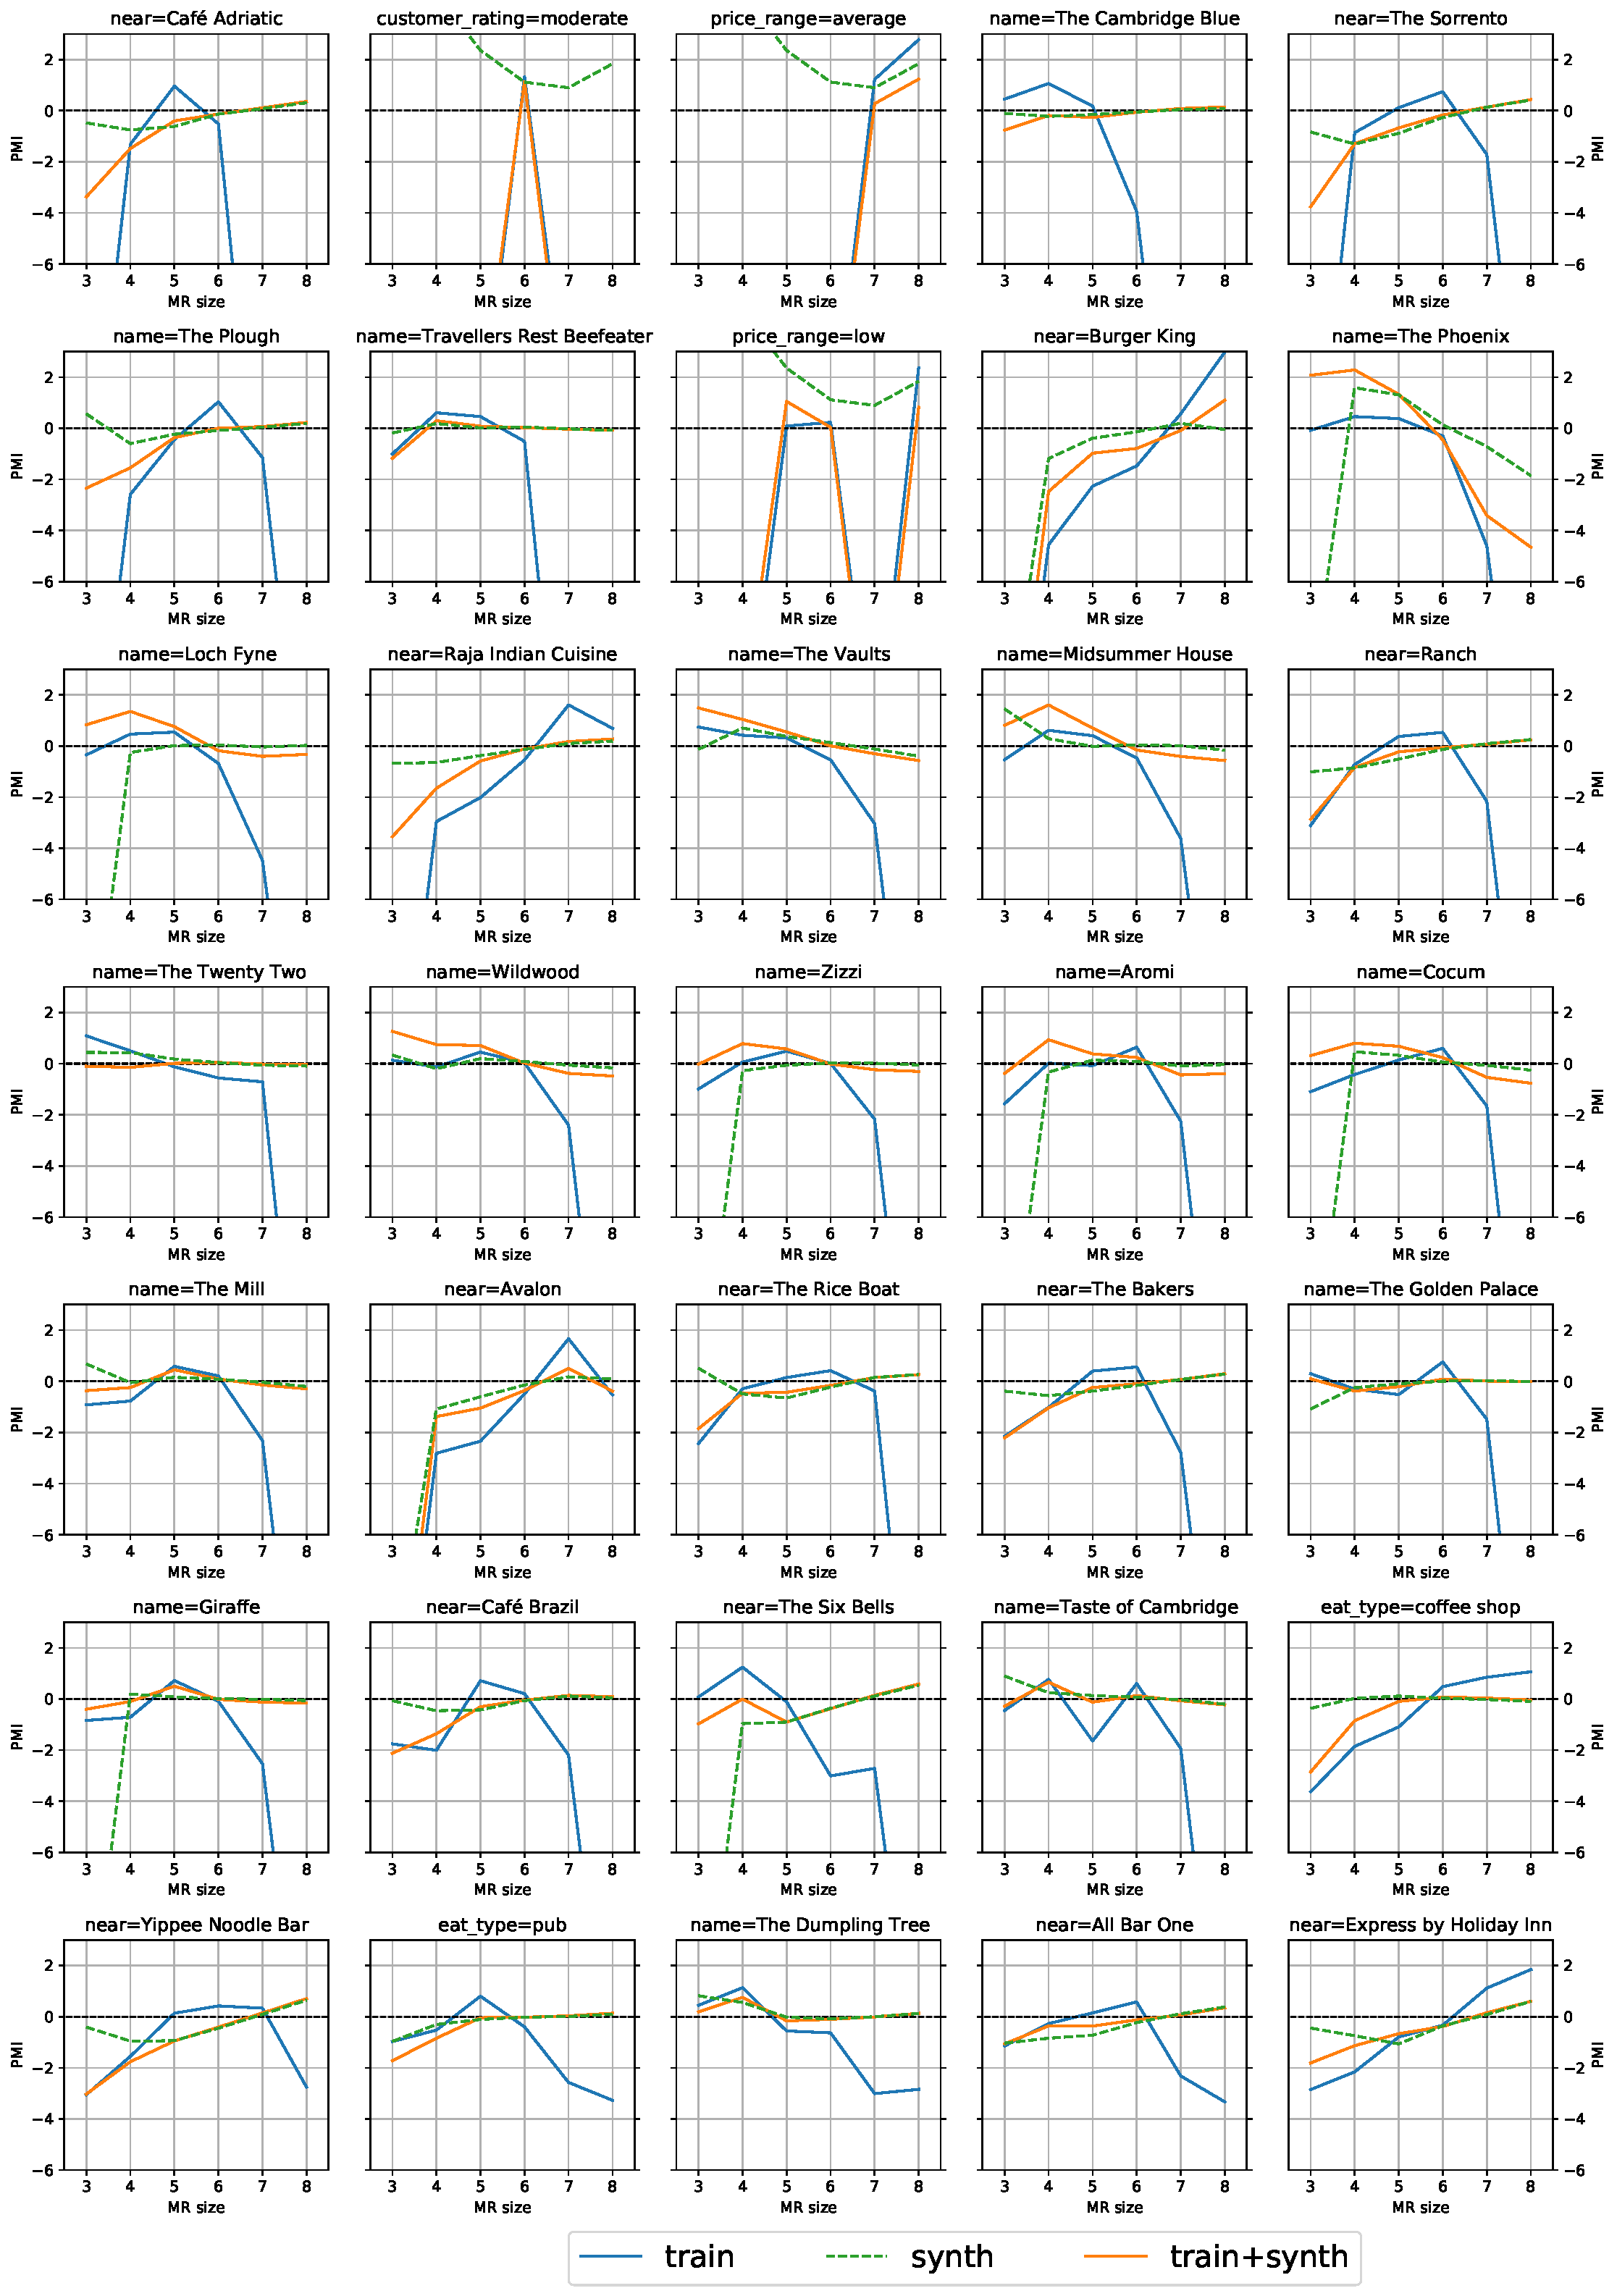
\includegraphics[width=0.9\textwidth]{ch5/figures/synthpmis.pdf}
\caption{PMI between various \attributevalue s and \meaningrepresentation~size
on the E2E Challenge dataset (blue), synthetic dataset (dashed green), and their union (orange). 0 on the $y$-axis indicates the two variables are independent.}
\label{fig:synthpmi}
\end{figure}


These recombinations are helpful. When we compare the PMI of various
\attributevalues~to \meaningrepresentation~size when using the original
training data (i.e., the plots we showed in \autoref{fig:bkpmi} and
\autoref{fig:trainpmi}) against the union of original and synthetic data
produced by noise-injection sampling (show in \autoref{fig:synthpmi}), we see
that most plots are much closer to 0 with the union of datasets, indicative of
greater independence between length and a particular \attributevalue, and that
this spurious association has been lessened considerably if not removed.

\begin{figure}
\begin{tikzpicture}
\node[anchor=north west,fill=olive,minimum height=2cm,text width=9cm] at (-8.1,3.90) {};
\node[anchor=north west,fill=violet,minimum height=2cm,text width=9cm] at (-8.1,3.75) {};
\node[anchor=north west,fill=blue,minimum height=2cm,text width=9cm] at (-8.1,3.23) {};
\node[anchor=north west,fill=purple,minimum height=2cm,text width=9cm] at (-8.1,3.0) {};
\node[anchor=north west,fill=green,minimum height=2cm,text width=9cm] at (-8.1,2.85) {};
\node[anchor=north west,fill=orange,minimum height=3cm,text width=9cm] at (-8.1,2.33) {};
\node[anchor=north west,fill=lime,minimum height=2cm,text width=9cm] at (-8.1,-.20) {};
\node[anchor=north west,fill=red,minimum height=0.59cm,text width=9cm] at (-8.1,-1.65) {};


\node[anchor=north west,fill=olive,minimum height=2cm,text width=0.1mm] at (0.33-7.35,-2.10) {};
\node[anchor=north west,fill=violet,minimum height=2cm,text width=2.8mm] at (0.48-7.35,-2.10) {};
\node[anchor=north west,fill=blue,minimum height=2cm,text width=2.8mm] at (1.0-7.35,-2.10) {};
\node[anchor=north west,fill=purple,minimum height=2cm,text width=2.8mm] at (1.22-7.35,-2.10) {};
\node[anchor=north west,fill=green,minimum height=2cm,text width=2.8mm] at (1.38-7.35,-2.10) {};
\node[anchor=north west,fill=orange,minimum height=2cm,text width=35.8mm] at (1.90-7.35,-2.10) {};
\node[anchor=north west,fill=lime,minimum height=2cm,text width=16.8mm] at (4.45-7.35,-2.10) {};
\node[anchor=north west,fill=red,minimum height=2cm,text width=3.3mm] at (5.86-7.35,-2.10) {};




\node[anchor=north west,fill=olive,minimum height=2cm,text width=0.1mm] at (0.33,-2.10) {};
\node[anchor=north west,fill=violet,minimum height=2cm,text width=2.8mm] at (0.48,-2.10) {};
\node[anchor=north west,fill=blue,minimum height=2cm,text width=2.8mm] at (1.0,-2.10) {};
\node[anchor=north west,fill=purple,minimum height=2cm,text width=2.8mm] at (1.22,-2.10) {};
\node[anchor=north west,fill=green,minimum height=2cm,text width=2.8mm] at (1.38,-2.10) {};
\node[anchor=north west,fill=orange,minimum height=2cm,text width=35.8mm] at (1.90,-2.10) {};
\node[anchor=north west,fill=lime,minimum height=2cm,text width=16.8mm] at (4.45,-2.10) {};
\node[anchor=north west,fill=red,minimum height=2cm,text width=3.3mm] at (5.86,-2.10) {};
\node at (0,0) {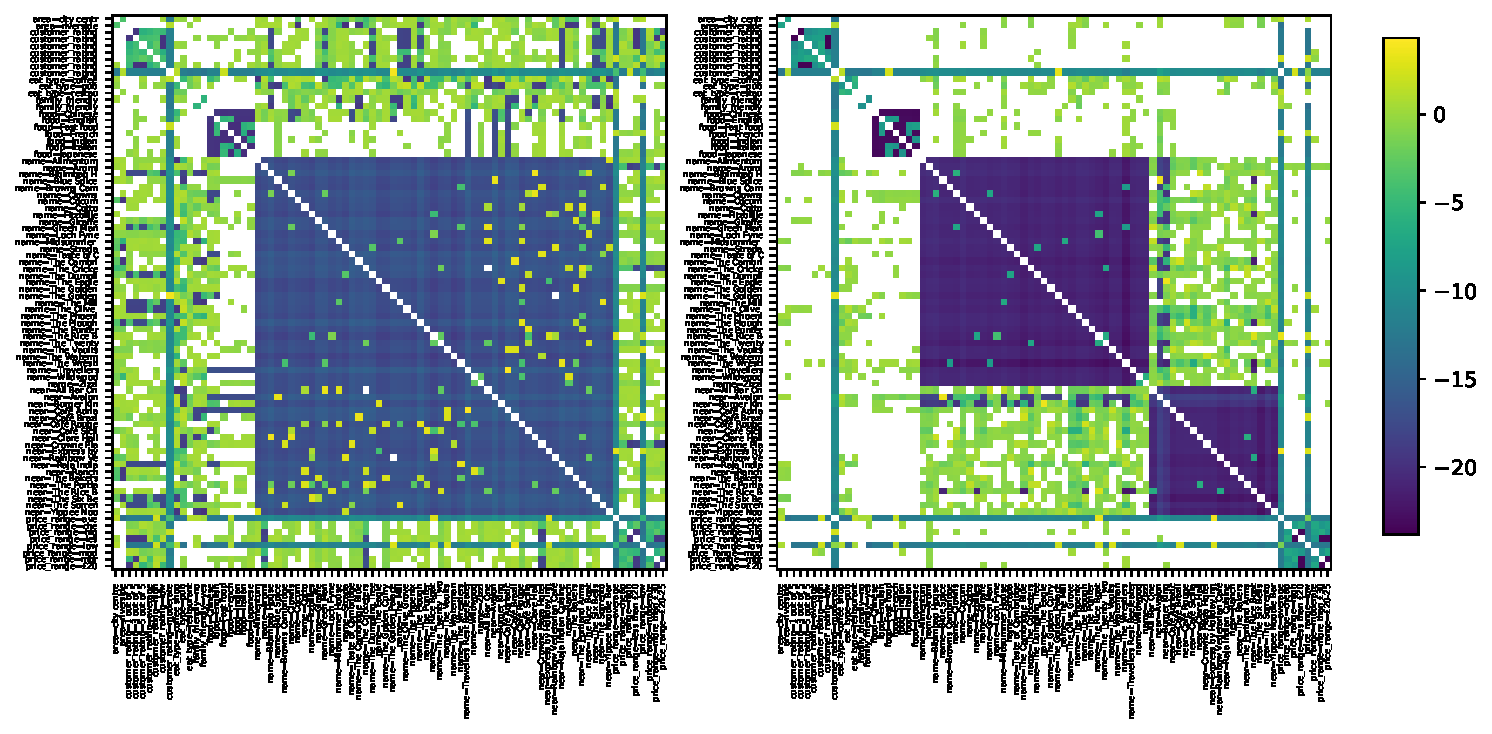
\includegraphics[width=\textwidth]{ch5/figures/heatmap_train.pdf}};
\end{tikzpicture}
\caption{PMI between E2E Challenge attribute-values on the original training data (left) and the union of the training and synthetic data (right). PMI between $(-.25,.25)$ are colored white and suggest relative independence between the two attribute-value pairs. Color blocks on the $x$ and $y$ axis labels correspond to groups of values for the same attribute. E.g., orange are all the values for the \Atr{name}~attribute.}
\label{fig:avpmi}
\end{figure}


Length is not the only spurious correlation present in the original training
dataset that can be mitigated by the synthetic datasets. In \autoref{fig:avpmi}
we plot the PMI between the occurrence of any two \attributevalues, e.g.
PMI(name=The Eagle,near=Burger King), on the original training data and union
of original and synthetic data.  Anti-correlation, i.e. extremely negative PMI
values, along the diagonal are expected as attribute-values in the E2E
Challenge dataset are mutually exclusive and don't usually co-occur (modulo
human annotator error).  We show PMI in the range of $(-.25, .25)$ as white
indicating roughly no strong association. In the ideal dataset, aside from
anti-correlation among values for the same attribute, we would like most the
PMI values to be close to 0. When comparing the PMI from the original dataset
(left) the union of original and synthetic, we see much more whitespace in the
latter suggesting there are fewer spurious associations between
\attributevalues~on the union dataset.

Producing training datasets with fewer spurious associations appears to be
highly beneficial when training \sequencetosequence~models for text generation
as we observe reduced semantic errors, and improved performance of greedy
decoding compared to more computationally intensive inference procedures.
